\documentclass[11pt,a4paper]{article}

% French
\usepackage[utf8x]{inputenc}
\usepackage[frenchb]{babel}
\usepackage[T1]{fontenc}
\usepackage{lmodern}
\usepackage{url}

% Math symbols
\usepackage{amsmath}
\usepackage{amssymb}
\usepackage{amsthm}
\usepackage{subfigure} %Allows to have several figures on the same line.
\usepackage{hyperref} %Allows to make references (\ref{}), pdf links are now clickable.
\usepackage{fmtcount} %Allows to use counters
\usepackage{fourier-orns} % Allows to display the \danger symbol
\usepackage{here} % Allows to place a figure where we want

\usepackage{makeidx} %Allows to create an index
\usepackage{enumerate} %Used where??
\makeindex
\usepackage[totoc]{idxlayout} %Allows to add the index in the table of contents

% Theorem and definitions
\theoremstyle{definition}
\newtheorem{mydef}{Définition}[subsection]
\newtheorem{mynota}[mydef]{Notation}
\newtheorem{myprop}[mydef]{Propriétés}
\newtheorem{myrem}[mydef]{Remarque}
\newtheorem{myform}[mydef]{Formules}
\newtheorem{mycorr}[mydef]{Corrolaire}
\newtheorem{mytheo}[mydef]{Théorème}
\newtheorem{mylem}[mydef]{Lemme}
\newtheorem{myexem}[mydef]{Exemple}
\newtheorem{myalgo}[mydef]{Algorithme}

\usepackage{algorithm}
\usepackage{algorithmic}

\newcommand{\bigoh}{\mathcal{O}}

\usepackage{tkz-graph}
\usepackage{tikz}
\usetikzlibrary{arrows,matrix,decorations.pathreplacing,positioning,chains,fit,shapes,calc} %Voir 1.3.8

\definecolor{mygreen}{rgb}{0,0.6,0}
\definecolor{mygray}{rgb}{0.5,0.5,0.5}
\definecolor{mymauve}{rgb}{0.58,0,0.82}

\tikzstyle{vertex}=[circle,fill=gray!50,minimum size=15pt,inner sep=0pt]
\tikzstyle{visited}=[circle,fill=green!25,minimum size=15pt,inner sep=0pt]
\tikzstyle{unvisited}=[circle,fill=blue!25,minimum size=15pt,inner sep=0pt]

\newcommand{\W}{\ {\color{red} \textbf{!!}} \ }
\newcommand{\degmax}{\deg_{\mathrm{max}}}

% Flots
\newcommand{\flotmax}{f_\mathrm{max}}
\DeclareMathOperator{\fnet}{f_\mathrm{net}}
\DeclareMathOperator{\coupe}{capacité}
\DeclareMathOperator{\coupemin}{\mathrm{coupe}_\mathrm{min}}
\DeclareMathOperator{\degin}{\deg_\mathrm{in}}
\DeclareMathOperator{\degout}{\deg_\mathrm{out}}
\DeclareMathOperator{\valeur}{valeur}
\DeclareMathOperator{\voisin}{Voisin}
\DeclareMathOperator{\vconn}{connectivité}
\DeclareMathOperator{\econn}{arête-connectivité}


\title{INMA1691 - Théorie et Algorithmique des Graphes}
\author{
  Robin Ballarini
  \and Annelies Bauwens
  \and Gilles Bertrand
  \and Armand Bosquillon de Jenlis
  \and Romain Capron
  \and Arnaud Cerckel
  \and Charlotte Cirriez
  \and Simon Claessens
  \and Gaëtan Collart
  \and Matthieu Constant
  \and Xavier Crochet
  \and Gatien De Callataÿ
  \and François Dederichs
  \and François Delcourt
  \and Arnaud de Lhoneux
  \and Martin De Neuville
  \and Guillaume Derval
  \and Alexandre de Touzalin
  \and Gauthier Feuillen
  \and Florentin Goyens
  \and Arnaud Jacques
  \and Antoine Hilhorst
  \and Benoît Legat
  \and Arthur Losseau
  \and Alexis Pierret
  \and Thérèse Plissart
  \and François Raucent
  \and Félicien Schiltz
  \and Mélanie Sedda
  \and Benoît Sluysmans
  \and Nicolas Stevens
  \and Harold Taeter
  \and Kim Van Den Eeckhaut
  \and Geoffroy Vanderreydt
  \and Antoine Van Malleghem
  \and Nicolas Vico}


\begin{document}

%%%%%%%%%%%%%%%%%%%%%%%%%%%%%%%%%%%%%%%%%%%%%%%%%%%%%%%%%%%%%%%
%%%%%%%%%%%%%%%%%%%%%%%% PAGE DE GARDE %%%%%%%%%%%%%%%%%%%%%%%%
%%%%%%%%%%%%%%%%%%%%%%%%%%%%%%%%%%%%%%%%%%%%%%%%%%%%%%%%%%%%%%%
\pagenumbering{gobble}% Remove page numbers
\maketitle
\begin{center}
  \vspace{-5mm}
  \textit{Basé sur le cours de Jean-Charles Delvenne}\\
  \includegraphics[width=100pt]{../img/logo}\\
  \textbf{Code source et bug tracker}\\
  \url{https://github.com/blegat/LINMA1691}
\end{center}
\newpage
\clearpage

%%%%%%%%%%%%%%%%%%%%%%%%%%%%%%%%%%%%%%%%%%%%%%%%%%%%%%%%%%%%%%%
%%%%%%%%%%%%%%%%%%%%%%% Table Of Contents %%%%%%%%%%%%%%%%%%%%%
%%%%%%%%%%%%%%%%%%%%%%%%%%%%%%%%%%%%%%%%%%%%%%%%%%%%%%%%%%%%%%%
\pagenumbering{arabic}% Arabic page numbers (and reset to 1)
\tableofcontents
\newpage

\newcounter{todo_1}
\newcounter{todo_2}
\newcounter{todo_3}
\newcounter{todo_4}
\newcounter{todo_5}
\newcounter{todo_6}
\newcounter{todo_7}
\newcounter{todo_8}
\newcounter{todo_9}
\newcounter{todo_10}
\newcounter{todo_11}
\newcounter{todo_12}

\newcommand{\addTODO}
{
  \textcolor{red}{TODO}\stepcounter{todo_\thesection}
}

\newcommand{\Chapitredone}[2]
{
  \ifnum#1=0
    Chapitre #2 terminé!
  \else
    \textbf{#1} dans le Chapitre #2
  \fi
}
\newcommand{\username}[2]
{
  \textit{\textbf{#1}} $\longleftrightarrow$ \textbf{#2}
}

\section{Graphes connexes, eulériens et bipartis }
\subsection{Graphes}

\index{graphe}
\begin{mydef}
  Un \emph{graphe} est un triplet ($V$, $E$, $\varphi$), où :
  \begin{itemize}
    \item $V$ est un ensemble dont les éléments sont appelés sommets ou noeuds;
    \item $E$ est un ensemble dont les éléments sont appelés arêtes;
    \item $\varphi$ est une fonction, dîte fonction d'incidence, qui associe à chaque arête un sommet ou une paire de sommets.
  \end{itemize}
\end{mydef}

\index{sommets adjacents}
\begin{mydef}
  Deux sommets incidents à la même arête sont dits \emph{adjacents}.
\end{mydef}

\index{boucle}
\begin{mydef}
  Une arête incidente à un seul sommet est une \emph{boucle}.
\end{mydef}

\index{degré}
\begin{mydef}
  Le \emph{degré} d'un sommet est le nombre d'arêtes incidentes à celui-ci.
\end{mydef}

\index{graphe!sous-graphe}
\begin{mydef}
  Un \emph{sous-graphe du graphe} ($V$, $E$, $\varphi$) est un graphe ($V'$, $E'$, $\varphi'$) avec :
  \begin{itemize}
    \item $V' \subseteq V$ ;
    \item $E' \subseteq E$ ;
    \item $\varphi'$ est la restriction de $\varphi'$ à $E'$.
  \end{itemize}
\end{mydef}

\index{isomorphisme}
\subsection{Isomorphisme de Graphes}
\begin{mydef}
  Deux graphes ($V$, $E$, $\varphi$) et ($V'$, $E'$, $\varphi'$) sont dits \emph{isomorphes} s'il existe des bijections $f:V \to V'$ et $g:E \to E'$ telles que :
  \begin{center}
    $\varphi(e) = \{u, v\}$ ssi $\varphi(g(e)) = \{f(u), f(v)\}$.
  \end{center}
  Deux graphes sont isomorphes s'il y a une bijection entre les noeuds et les arêtes.
\end{mydef}

\begin{myexem}
  Voici deux exemples d'isomorphisme du même graphe :
    \begin{figure} [!h]
      \centering
	    \subfigure[]
    	{
    	  \begin{tikzpicture}[scale = 0.75]
          \node[draw, circle] at ( 0, 1.5)  (1) {1};
          \node[draw, circle] at ( 2, 0  )  (2) {2};
          \node[draw, circle] at ( 1,-1.5)  (3) {3};
          \node[draw, circle] at (-1,-1.5)  (4) {4};
          \node[draw, circle] at (-2, 0  )  (5) {5};

          \draw[-] (1) edge [bend left] node[anchor = south] {a} (2);
          \draw[-] (2) edge [bend left] node[anchor = west]  {b} (3);
          \draw[-] (3) edge [bend left] node[anchor = north] {c} (4);
          \draw[-] (4) edge [bend left] node[anchor = east]  {d} (5);
          \draw[-] (5) edge [bend left] node[anchor = east]  {e} (1);
        \end{tikzpicture}
      }
      % Cette ligne de commentaire semble être nécessaire pour que les figures soient affichées sur une ligne
      \subfigure[]
      {
        \begin{tikzpicture}[scale = 0.75]
          \node[draw, circle] at ( 0, 1.5)  (1) {$1'$};
          \node[draw, circle] at ( 2, 0.5)  (2) {$2'$};
          \node[draw, circle] at ( 1,-1.5)  (3) {$3'$};
          \node[draw, circle] at (-1,-1.5)  (4) {$4'$};
          \node[draw, circle] at (-2, 0.5)  (5) {$5'$};

          \draw[-] (1) edge [bend left] node[pos=0.05, anchor = west] {$a'$} (3);
          \draw[-] (2) edge node[anchor = north] {$b'$} (5);
          \draw[-] (2) edge node[pos=0.5, anchor = west] {$c'$} (4);
          \draw[-] (3) edge node[pos=0.5, anchor = east] {$d'$} (5);
          \draw[-] (1) edge [bend right] node[pos=0.05, anchor = east] {$e'$} (4);

        \end{tikzpicture}
      }
      % Cette ligne de commentaire semble être nécessaire pour que les figures soient affichées sur une ligne
      \subfigure[]
      {
        \begin{tikzpicture}[scale = 0.75]
          \node[draw, circle] at ( 0, 1.5)  (1) {$1'$};
          \node[draw, circle] at ( 2, 0  )  (4) {$4'$};
          \node[draw, circle] at ( 1,-1.5)  (2) {$2'$};
          \node[draw, circle] at (-1,-1.5)  (5) {$5'$};
          \node[draw, circle] at (-2, 0  )  (3) {$3'$};

          \draw[-] (1) edge [bend left] node[anchor = south] {$e'$} (4);
          \draw[-] (4) edge [bend left] node[anchor = west]  {$c'$} (2);
          \draw[-] (2) edge [bend left] node[anchor = north] {$b'$} (5);
          \draw[-] (5) edge [bend left] node[anchor = east]  {$d'$} (3);
          \draw[-] (3) edge [bend left] node[anchor = east]  {$a'$} (1);
        \end{tikzpicture}
      }
    \end{figure}
    Notons que les graphes \emph{b} et \emph{c} sont les mêmes, leurs noeuds ont simplement été réordonnés.\\
    L'isomorphisme entre \emph{a} et les deux autres est donné par : \\

    \begin{tabular}{lll}
      $f(1)=1'$ & $g(a)=e'$ \\
      $f(2)=4'$ & $g(b)=c'$ & $\varphi(a) = \{1, 2\}$\\
      $f(3)=2'$ & $g(c)=b'$ & $\varphi'(a') = \{1', 3'\}$\\
      $f(4)=5'$ & $g(d)=d'$ & $\varphi'(g(a)) = \{f(1), f(2)\}$\\
      $f(5)=3'$ & $g(e)=a'$ \\
    \end{tabular}
    \newline
    \newline
    Notons aussi que plusieurs résultats sont possibles : \\
    \begin{figure}[!h]
      \centering
      \subfigure[]
      {
        \begin{tikzpicture}[scale = 0.75]
          \node[draw, circle] at ( 0, 1.5)  (1) {1};
          \node[draw, circle] at ( 2, 0  )  (2) {2};
          \node[draw, circle] at ( 1,-1.5)  (3) {3};
          \node[draw, circle] at (-1,-1.5)  (4) {4};
          \node[draw, circle] at (-2, 0  )  (5) {5};

          \draw[-] (1) edge [bend left] node[anchor = south] {a} (2);
          \draw[-] (2) edge [bend left] node[anchor = west]  {b} (3);
          \draw[-] (3) edge [bend left] node[anchor = north] {c} (4);
          \draw[-] (4) edge [bend left] node[anchor = east]  {d} (5);
          \draw[-] (5) edge [bend left] node[anchor = east]  {e} (1);
        \end{tikzpicture}
      }
      % Cette ligne de commentaire semble être nécessaire pour que les figures soient affichées sur une ligne
      \subfigure[]
      {
        \begin{tikzpicture}[scale = 0.75]
          \node[draw, circle] at ( 0, 1.5)  (1) {$1'$};
          \node[draw, circle] at ( 2, 0.5)  (2) {$2'$};
          \node[draw, circle] at ( 1,-1.5)  (3) {$3'$};
          \node[draw, circle] at (-1,-1.5)  (4) {$4'$};
          \node[draw, circle] at (-2, 0.5)  (5) {$5'$};

          \draw[-] (1) edge [bend left] node[pos=0.05, anchor = west] {$a'$} (3);
          \draw[-] (2) edge node[anchor = north] {$b'$} (5);
          \draw[-] (2) edge node[pos=0.5, anchor = west] {$c'$} (4);
          \draw[-] (3) edge node[pos=0.5, anchor = east] {$d'$} (5);
          \draw[-] (1) edge [bend right] node[pos=0.05, anchor = east] {$e'$} (4);

          %TODO tracer les lignes qui montrent comment on passe du graphe e au graphe f (en gardant les 3 graphes sur la même ligne)
        \end{tikzpicture}
      }
      % Cette ligne de commentaire semble être nécessaire pour que les figures soient affichées sur une ligne
      \subfigure[]
      {
        \begin{tikzpicture}[scale = 0.75]
          \node[draw, circle] at ( 0, 1.5)  (1) {$1'$};
          \node[draw, circle] at ( 2, 0  )  (3) {$3'$};
          \node[draw, circle] at ( 1,-1.5)  (5) {$5'$};
          \node[draw, circle] at (-1,-1.5)  (2) {$2'$};
          \node[draw, circle] at (-2, 0  )  (4) {$4'$};

          \draw[-] (1) edge [bend left] node[anchor = south] {$a'$} (3);
          \draw[-] (3) edge [bend left] node[anchor = west]  {$b'$} (5);
          \draw[-] (5) edge [bend left] node[anchor = north] {$d'$} (2);
          \draw[-] (2) edge [bend left] node[anchor = east]  {$c'$} (4);
          \draw[-] (4) edge [bend left] node[anchor = east]  {$e'$} (1);
        \end{tikzpicture}
      }
    \end{figure}

    \begin{tabular}{lll}
      $f(1)=1'$ & $g(a)=a'$ \\
      $f(2)=3'$ & $g(b)=b'$ \\
      $f(3)=5'$ & $g(c)=d'$ \\
      $f(4)=2'$ & $g(d)=c'$ \\
      $f(5)=4'$ & $g(e)=e'$ \\
    \end{tabular}
    \newline
    \newline
    Les six graphes de cet exemple sont isomorphes entre eux.\\
\end{myexem}

\subsection{Parcours eulérien}
\index{parcours}
\begin{mydef}%TODO définir ce qu'est un parcours
  Un \emph{parcours} est fermé si $v_0 = v_1$.
\end{mydef}

\index{chemin}
\begin{mydef}
  Un \emph{chemin} est un parcours dont tous les sommets sont distincts.
\end{mydef}

\index{cycle}
\begin{mydef}
  Un \emph{cycle} est un parcours fermé dont tous les sommets d'origine et intérieurs sont tous distincts.
\end{mydef}

\index{graphe!graphe connexe}
\begin{mydef}
  Un \emph{graphe} est \emph{connexe} si pour chaque pair de points il existe un parcours qui les relie. Les \emph{composantes connexes} d'un graphe sont ses sous-graphes connexes maximaux.
\end{mydef}

\index{parcours!parcours eulérien}
\index{graphe!graphe eulérien}
\begin{mydef}
  Un \emph{parcours} est \emph{eulérien} s'il visite chaque arête une et une seule fois. Un \emph{graphe} est \emph{eulérien} s'il existe un parcours eulérien fermé.
\end{mydef}

\begin{mytheo} [Théorème d'Euler]
  Un graphe connexe est eulérien ssi tous les sommets sont de degré pair.
  \begin{proof}
    \noindent
    \newline
    \fbox{$\Longrightarrow$}
    \newline
    Chaque arête incidente à un noeud $x$ est utilisé par le parcours eulérien:
    \begin{itemize}
      \item soit pour entrer dans $x$;
      \item soit pour en sortir.\\
    \end{itemize}
    A chaque arête entrante correspond une arête sortante (celle qui suit dans le parcours sauf pour la dernière et la première).\\
    Donc, il y a une bijection entre les arêtes entrantes et les arêtes sortantes.\\
    $\longrightarrow$ degré pair \\

    \noindent
    \fbox{$\Longleftarrow$}
    \newline
    On va construire un parcours eulérien :\\
    \begin{enumerate}
      \item On part d'un noeud arbitraire $x_0$.
      \item On prend une arête incidente à $x_0$, on arrive à un nouveau noeud.
      \item Par parité, il y a au moins une arête non utilisée, on la prend, etc... Quand il n'y a plus d'arête disponible, on est forcément arrivé à $x_0$.\\
    \end{enumerate}
    \begin{center}
      \begin{tikzpicture}[scale = 0.75]
        \node[draw, circle] at (-3, 0  )  (1)  {$x_0$};
        \node[draw, circle] at (-2, 1.5)  (2)  {};
        \node[draw, circle] at (-2,-1.5)  (3)  {};
        \node[draw, circle] at (-1, 0  )  (4)  {};
        \node[draw, circle] at ( 0, 1.5)  (5)  {};
        \node[draw, circle] at ( 0,-1.5)  (6)  {};
        \node[draw, circle] at ( 1, 0  )  (7)  {$x_1$};
        \node[draw, circle] at ( 2, 1.5)  (8)  {};
        \node[draw, circle] at ( 2,-1.5)  (9)  {};
        \node[draw, circle] at ( 3, 0  )  (10) {};

        \draw[-] (1) edge node {} (2);
        \draw[dotted] (1) edge node {} (3);
        \draw[-] (2) edge node {} (4);
        \draw[-] (3) edge node {} (4);
        \draw[-] (4) edge node {} (5);
        \draw[-] (4) edge node {} (6);
        \draw[-] (5) edge node {} (7);
        \draw[-] (6) edge node {} (7);
        \draw[-] (7) edge node {} (8);
        \draw[-] (7) edge node {} (9);
        \draw[-] (8) edge node {} (10);
        \draw[-] (9) edge node {} (10);
      \end{tikzpicture}
    \end{center}
    Pour tout autre noeud y, en arrivant à y, on a utilisé un nombre impair d'arêtes incidentes à y. On a un parcours fermé :
    \begin{itemize}
      \item Si toutes les arêtes incidentes aux x noeuds traversés par ce parcours sont utilisées, alors ce parcours est eulérien;
      \item Sinon, il y a $x_1 \in$ parcours avec au moins une arête non exploitée.\\
    \end{itemize}
    \begin{center}
      \begin{tikzpicture}[scale = 0.75]
        \node[draw, circle] at (-4, 0  )  (1)  {};
        \node[draw, circle] at (-4,-1.5)  (2)  {};
        \node[draw, circle] at (-2, 0  )  (3)  {$x_0$};
        \node[draw, circle] at (-2,-1.5)  (4)  {};
        \node[draw, circle] at (-2, 1.5)  (5)  {};
        \node[draw, circle] at ( 0, 1.5)  (6)  {};
        \node[draw, circle] at ( 0, 0  )  (7)  {$x_1$};
        \node[draw, circle] at ( 0,-1.5)  (8)  {};
        \node[draw, circle] at ( 2,-1.5)  (9)  {};
        \node[draw, circle] at ( 2, 0  )  (10) {};

        \draw[-] (1) edge node {} (2);
        \draw[-] (1) edge node {} (3);
        \draw[-] (2) edge node {} (4);
        \draw[-] (3) edge node {} (4);
        \draw[-] (3) edge node {} (5);
        \draw[-] (3) edge node {} (7);
        \draw[-] (5) edge node {} (6);
        \draw[-] (6) edge node {} (7);
        \draw[-, color=red] (7) edge node {} (8);
        \draw[-, color=red] (7) edge node {} (10);
        \draw[-, color=red] (8) edge node {} (9);
        \draw[-, color=red] (9) edge node {} (10);
      \end{tikzpicture}
    \end{center}
    On merge les deux parcours :\\
    $P_{0+1} = x_0 \rightarrow x_1 \textcolor{red}{\rightarrow} x_1 \rightarrow x_0$\\
    Et on fait ça en boucle jusqu'à avoir toutes les arêtes.
  \end{proof}
\end{mytheo}

\begin{mytheo} [Existence d’un parcours eulérien]
  Un graphe connexe possède un parcours eulérien ssi le nombre de noeuds de degré impair est zéro ou deux.
  \begin{proof}
    \noindent
    \newline
    \fbox{$\Longrightarrow$}
    \newline
    \begin{itemize}
      \item Si ce parcours eulérien est fermé, tous les degrés sont pairs;
      \item Si ce parcours eulérien est ouvert, tous les degrés sont pairs, sauf $deg(u)$ et $deg(v)$ qui sont impairs.\\
    \end{itemize}

    \noindent
    \fbox{$\Longleftarrow$}
    \newline
    \begin{itemize}
      \item Si tous les degrés sont pairs alors il existe un parcours eulérien fermé;
      \item Si deux degrés sont impairs et si on ajoute une arête $e$ entre $u$ et $v$ :\\
      $\rightarrow$ Tous les degrés sont pairs.\\
      $\rightarrow$ Il existe un parcours eulérien fermé.\\
      En retirant $e$, on obtient un parcours eulérien ouvert $u \rightarrow v$
    \end{itemize}
  \end{proof}
\end{mytheo}

\begin{mytheo} [Théorème des poignées de mains]
  La somme des degrés des noeuds d’un graphe est deux fois le nombre d’arêtes.\\
  $\sum_{v_i \in V}^{} deg(v_i) = 2|E|$
  \begin{proof}
    En utilisant la matrice d'incidence $M$ (voir \ref{in_matrix}), on peut calculer $\sum_{i,j}^{} M_{i,j}$ de deux façon différentes :\\
    \begin{tikzpicture}[decoration=brace]
      \matrix (m) [matrix of math nodes,left delimiter=[,right delimiter={]}] {
          0 & 1 & 1 & 0 & 1 & 0 \\
          1 & 1 & 0 & 1 & 0 & 1 \\
          1 & 0 & 0 & 1 & 0 & 1 \\
          0 & 0 & 1 & 0 & 1 & 0 \\
      };
      \draw[decorate,transform canvas={xshift=1.3em},thick] (m-1-6.north east) -- node[right=2pt] {$\sum_i \sum_j M_{ij} = \sum_{v_i \in V} deg(v_i)$} (m-4-6.south east);
      \draw[decorate,transform canvas={yshift=-1.7em},thick] (m-4-6.north east) -- node[below=2pt] {$\sum_i \sum_j M_{ij} = 2|E|$} (m-3-1.south west);
    \end{tikzpicture}
    \vspace*{5mm}
    \begin{center}
      $\sum_i \sum_j M_{ij} = \sum_i \sum_j M_{ij}$\\
      \vspace*{2mm}
      $2|E| = \sum_{v_i \in V} deg(v_i)$
    \end{center}
  \end{proof}
\end{mytheo}

\subsection{Représentation matricielle du graphe}
\index{matrice d'adjacence}
\begin{mydef}
  La \emph{matrice d'adjacence} est une matrice carrée $n$x$n$ dont l'élément $ij$ est le nombre d'arêtes entre les sommets $v_i$ et $v_j$.
\end{mydef}

\index{matrice d'incidence}
\begin{mydef}
  \label{in_matrix}
  La \emph{matrice d'incidence} est une matrice rectangulaire $n$x$m$ dont l'élément $ij$ est le nombre de fois que le sommet $v_i$ est incident à l'arête $e_j$.
\end{mydef}

\begin{myexem}
  \noindent
  \begin{center}
    \begin{tikzpicture}[scale = 0.75]
      \node[draw, circle] at ( 0, 4)  (1)  {$1$};
      \node[draw, circle] at ( 2, 0)  (2)  {$2$};
      \node[draw, circle] at (-2, 0)  (3)  {$3$};

      \draw[-] (1) edge [loop above] node {a} (1);
      \draw[-] (1) edge [bend left] node [anchor = north] {b} (2);
      \draw[-] (1) edge [bend right] node [anchor = north] {c} (2);
      \draw[-] (2) edge node [anchor = north] {d} (3);
      \draw[-] (1) edge node [anchor = north] {e} (3);
    \end{tikzpicture}

    $
    Matrice\ d'adjacence\ :\ A\ = \bordermatrix{~ & 1 & 2 & 3 \cr
                                                1 & 1 & 2 & 1 \cr
                                                2 & 2 & 0 & 1 \cr
                                                3 & 1 & 1 & 0 \cr}
    $

    $
    Matrice\ d'incidence\ :\ M\ = \bordermatrix{~ & a & b & c & d & e\cr
                                                1 & 2 & 1 & 1 & 0 & 1\cr
                                                2 & 0 & 1 & 1 & 1 & 0\cr
                                                3 & 0 & 0 & 0 & 1 & 1\cr}
    $
  \end{center}
  $(A^k)_{ij} =$ nombre de parcours $i \to j$ de longueur $k$.\\
  $
    A^0\ =\ I\ =  \begin{pmatrix} 1 & 0 & 1\\
                                  0 & 1 & 0\\
                                  0 & 0 & 1
                  \end{pmatrix},\
    A^1\ =\ A\ =\begin{pmatrix} 1 & 2 & 1\\
                                2 & 0 & 1\\
                                1 & 1 & 0
                \end{pmatrix},\
    A^2\ = \begin{pmatrix}  6 & 3 & 3\\
                            3 & 5 & 2\\
                            3 & 2 & 2
            \end{pmatrix}
  $
\end{myexem}

\begin{mytheo} [Matrice d’adjacence et nombre de parcours]
  Soit $A$ la matrice d'adjacence d'un graphe. Alors l'élément $ij$ de $A^k$ ($k \geq 0$) est le nombre de parcours de longueur $k$ de $v_i$ vers $v_j$.
  \begin{proof}
    Nous procédons par récurrence. Soit $A$ une matrice d'adjacence.\\
    Pour $k=0$, $A^{0}=Id$. La propriété est vérifiée par convention. Il existe un chemin de longueur 0 d'un point vers lui même. \\
    Pour $k=1$, $A^{1}=A$ représente bien le nombre de parcours de longueur 1. \\
    Supposons la propriété vérifiée pour $A^{k}$.

    Nombre de parcours de parcours de $i \to j$ de longueur $k+1 =$\\
    $= \sum_{l \in E}$ (\# parcours de $i \to l$ de longueur $k$)$.$(\# arêtes $l \to j$)\\
    $= \sum_{l \in E} A_{il}^{k}.A_{lj}$\\
    $= A_{ij}^{k+1}$
  \end{proof}
\end{mytheo}

\index{distance entre deux noeuds}
\begin{mydef}
  La \emph{distance $d(u, v)$} entre les noeuds $u$ et $v$ d'un graphe est le nombre d'arêtes minimal d'un parcours entre ces deux noeuds.
\end{mydef}

\begin{mylem}
  Si $u...u'...v'...v$ est un parcours de longeur minimale de $u$ vers $v$, alors le sous-parcours $u'...v'$ est un parcours de longeur minimale de $u'$ vers $v'$.\\
  En particulier, un parcours de longueur minimale est toujours un chemin.
  \begin{proof}
    Si ce parcours entre $u'$ et $v'$ n'était pas le plus court, on utiliserait le parcours strictement plus court pour la construction du parcours entre $u$ et $v$.
  \end{proof}
\end{mylem}

\subsection{Graphe biparti}
\index{graphe!graphe biparti}
\begin{mydef}
  Un graphe est \emph{biparti}  s'il existe une partition en deux ensembles $V_1$ et $V_2$ tels que les sommets de $V_1$ ne sont adjacents qu'à des sommets de $V_2$ et vice versa. La bipartition est $(V_1, V_2)$.
\end{mydef}

\begin{myexem}
  \noindent
  \begin{center}
    \definecolor{myblue}{RGB}{80,80,160}
    \definecolor{mygreen}{RGB}{80,160,80}

    \begin{tikzpicture}[thick,
      every node/.style={draw,circle},
      fsnode/.style={fill=myblue},
      ssnode/.style={fill=mygreen},
      every fit/.style={ellipse,draw,inner sep=-2pt,text width=2cm},
      ->,shorten >= 3pt,shorten <= 3pt
    ]

    % the vertices of U
    \begin{scope}[start chain=going below,node distance=7mm]
    \foreach \i in {1,2,...,5}
      \node[fsnode,on chain] (f\i) [label=\i] {};
    \end{scope}

    % the vertices of V
    \begin{scope}[xshift=4cm,yshift=-0.5cm,start chain=going below,node distance=7mm]
    \foreach \i in {6,7,...,9}
      \node[ssnode,on chain] (s\i) [label=\i] {};
    \end{scope}

    % the set U
    \node [myblue,fit=(f1) (f5),label=$V_1$] {};
    % the set V
    \node [mygreen,fit=(s6) (s9),label=$V_2$] {};

    % the edges
    \draw (f1) -- (s6);
    \draw (s6) -- (f2);
    \draw (f2) -- (s7);
    \draw (s7) -- (f3);
    \draw (s8) -- (f3);
    \draw (f3) -- (s9);
    \draw (s9) -- (f5);
    \draw (f5) -- (s6);
    \draw (f4) -- (s9);
    \end{tikzpicture}
  \end{center}
\end{myexem}

\begin{mytheo} [Graphes bipartis]
  Un graphe est biparti ssi tous ses cycles sont de longueur paire.
  \begin{proof}
    \noindent
    \newline
    \fbox{$\Longrightarrow$}
    \newline
    Il existe une bipartition $(V_1,V_2)$.\\
    \begin{align*}
      Cycle : & V_1, V_2, V_3, ..., V_n \Rightarrow n\ est\ pair.\\
              & \downarrow\ \ \ \downarrow\ \ \ \downarrow\ \ \ \ \ \ \ \downarrow\\
              & V_1, V_2, V_1, ..., V_2
    \end{align*}

    \noindent
    \fbox{$\Longleftarrow$}
    \newline
    Partition d'un noeud $v_0$ au hasard.\\
    $V_0\ =\ \{v|d(v,\ v_0)\ $paire$\}$\\
    $V_1\ =\ \{v|d(v,\ v_0)\ $impaire$\}$\\
    C'est une partition. Est-ce une bipartition?
    Oui, sinon on aurait par exemple une arête $uv$ dans $V_0$.

    \begin{center}
      \begin{tikzpicture}
        \node[draw, circle] at (-4, 0)  (1)  {$v_0$};
        \node[draw, circle] at (-1, 0)  (2)  {$w$};
        \node[draw, circle] at ( 2, 1)  (3)  {$u$};
        \node[draw, circle] at ( 2,-1)  (4)  {$v$};

        \draw[-] (1) edge [bend left]  node {} (2);
        \draw[-] (1) edge [bend right] node {} (2);
        \draw[-, color=red] (2) edge [bend left]  node [anchor = south, color=black] {pcc $v_0 \to u$} (3);
        \draw[-, color=red] (2) edge [bend right] node [anchor = north, color=black] {pcc $v_0 \to v$} (4);
        \draw[-, color=red] (3) edge node {} (4);
      \end{tikzpicture}
    \end{center}
    pcc : plus court chemin.\\
    Les pcc sont de longueure paire car on est dans $V_0$.\\
    $w$ est le dernier point d'intersection entre les chemins $v_0 \to u$ et $v_0 \to v$.\\
    \textcolor{red}{$\triangle$} est un cycle de longueur impaire car $w \to u$ et $w \to v$ sont paires (les deux sous-chemins de $v_0 \to w$ sont des plus court chemin de même longueur) + une arête $uv$.\\
    $lg(wuvw)\ =\ lg(v_{0}uvv_0)\ - \ 2lg(v_0w)$\\
    $impaire\ \ \ \ \ \ \ \ \ \ \ \ \ \ \ \ \ \ \ \ \ \ \ \ \ \ \ \ \ \ paire$\\
    Contradiction, si arête dans $V_1$ même raisonnement.
  \end{proof}
\end{mytheo}

\section{Les plus courts chemins}
\subsection{Les plus courts chemins}
\index{graphe!graphe pondéré}
\begin{mydef}
  Une \emph{fonction de poids} sur un graphe ($V$, $E$, $\varphi$) est une fonction $E \to \mathbb{R}$. Un \emph{graphe pondéré} est un graphe muni d’une fonction de poids. Le \emph{poids} ou la \emph{longueur} d’un parcours est la somme des poids des arêtes qui le compose.
\end{mydef}

\begin{mytheo} [Plus court chemin et plus court parcours]
  Pour un graphe avec une fonction de poids $\geq 0$, si le plus court parcours entre $u$ et $v$ est de longueur $d$, alors le plus court chemin entre $u$ et $v$ est aussi de longueur $d$.
  \begin{proof}
     Cette démonstration n'a pas été vue au cours.
  \end{proof}
\end{mytheo}

\subsection{Algorithme de Dijkstra}
\index{algorithme!algorithme de Dijkstra}
\begin{myalgo}[Algorithme de Dijkstra]
\noindent
\begin{enumerate}
  \item Initialement, $i=0$, l'ensemble $S={u_{0}}$ (il contient notre noeud de départ) et l'ensemble \={S}$_{0}$ contient tous les autres noeuds. $l(u_{0})=0$ et $l(v)=\infty$ pour $v\ne u_{0}$ ($l(v)$ est une borne supérieure de $d(u_{0},v)$).
	\item Pour chaque $v \in$ \=S$_{i}$, on remplace $l(v)$ par min $({l(v),l(u_{i}+w{u_{i}v)}})$. On calcule le minimum pour $v \in$\=S$_{i}$ de $l(v)$ et on nomme $u_{i+1}$ le sommet pour qui ce minimum est atteind. Ensuite, on fixe $S_{i+1}=S_{i} \cup {u_{i+1}}$ et on retire ce sommet de \=S$_{i+1}$.
	\item si $i=v-1$, on arrête. Si $i < v-1$, on remplace i par $i+1$ et on refait l'étape 2.
	\end{enumerate}
\end{myalgo}

\begin{myexem}
  On cherche les distances à partir de $a$.\\
	\begin{center}
	  \begin{tikzpicture}
      \node[vertex] at (0,  2) (a) {$a$};
      \node[vertex] at (2,  1) (b) {$b$};
      \node[vertex] at (1, -2) (c) {$c$};
      \node[vertex] at (-1,-2) (d) {$d$};
      \node[vertex] at (-2, 1) (e) {$e$};
      \draw[->] (a) edge node[anchor = south] {\tiny $50$} (b);
  		\draw[->] (c) edge node[anchor = north] {\tiny $5$} (b);
  		\draw[->] (c) edge node[anchor = north] {\tiny $50$} (d);
  		\draw[->] (e) edge node[anchor = south] {\tiny $10$} (d);
  		\draw[->] (a) edge node[anchor = south] {\tiny $10$} (e);
  		\draw[->] (d) edge node[anchor = north] {\tiny $5$} (a);
  		\draw[->] (a) edge node[anchor = south] {\tiny $30$} (c);
  		\draw[->] (d) edge node[anchor = north] {\tiny $20$} (b);
  	\end{tikzpicture}
  \end{center}
  \begin{center}
    \begin{tabular}{|c|c|ccccc|}
      \hline
      $u'$ & $S$ & $l(a)$ & $l(b)$ & $l(c)$ & $l(d)$ & $l(e)$\\
      \hline
      $a$ & $\lbrace a \rbrace$ & $\boxed{0}$ & $\infty$ & $\infty$ & $\infty$ &$\infty$\\
      $a$ & $\lbrace a,e \rbrace$ && 50 & 30 & $\infty$ & $\boxed{10}$\\
      $e$ & $\lbrace a,e,d \rbrace$ && 50 & 30 & $\boxed{20}$ &\\
      $d$ & $\lbrace a,e,d,c \rbrace$ && 40 & $\boxed{30}$ & &\\
      $c$ & $\lbrace a,e,d,c,b \rbrace$ && $\boxed{35}$ & & &\\
      \hline
    \end{tabular}
  \end{center}
\end{myexem}

\begin{mytheo} [L'algorithme de Dijkstra fonctionne]
  Après chaque MISE A JOUR DE $\ell$ dans l’algorithme, les deux propriétés suivantes sont vérifiées :
  \begin{itemize}
    \item pour $v \in S$, $\ell(v) = d(u_0, v)$ et le chemin le plus court de $u_0$ à $v$ reste dans $S$;
    \item pour $v \notin S$, $\ell(v) \geq d(u_0, v)$, et $\ell(v)$ est la longueur du plus court chemin de $u_0$ vers $v$ dont tous les noeuds internes sont dans $S$.
  \end{itemize}
  \begin{proof}
     Cette démonstration n'a pas été vue au cours.
  \end{proof}
\end{mytheo}

\begin{mycorr} [L'algorithme de Dijkstra est correct]
  L’algorithme de Dijkstra est correct.
\end{mycorr}

\begin{mytheo} [L’algorithme de Dijkstra est quadratique]
  L’algorithme de Dijkstra sur un graphe se termine en un temps de l’ordre $n^2$ .
  \begin{proof}
    \noindent
    \begin{itemize}
		\item A chaque passage de boucle $\left\lbrace v \in S \right\rbrace $ décroit de 1. Ce qui implique $n$ passages de boucles.
		\item A chaque boucle, "$\forall v \in S$" fait $O(n-|S|)$ opérations; et "trouver $v_{min}$" fait $O(n-|S|)$ opérations également.
		\item Cela implique un temps total $O(n + (n-1) + (n-2) + ... + 1) = O\left( \frac{n(n-1)}{2} \right) = O(n^2)$ puisqu'on considère le temps à une constante près.
		\end{itemize}
  \end{proof}
\end{mytheo}

\index{graphe!graphe dirigé}
\begin{mydef}
  Un \emph{graphe dirigé} est un triplet ($V$, $E$, $\varphi$), où :\\
  - $V$ est un ensemble dont les éléments sont appelés sommets ou noeuds; \\
  - $E$ est un ensemble dont les éléments sont appelés arêtes; \\
  - $\varphi$ est une fonction, dîte fonction d'incidence, qui associe à chaque arête un couple ordonné de sommets. \\
\end{mydef}

\begin{myexem}
Pour le graphe dirigé suivant :
  \begin{center}
	  \begin{tikzpicture}
      \node[vertex] at (0,  2) (a) {$a$};
      \node[vertex] at (2,  1) (b) {$b$};
      \node[vertex] at (1, -2) (c) {$c$};
      \node[vertex] at (-1,-2) (d) {$d$};
      \node[vertex] at (-2, 1) (e) {$e$};
      \draw[->] (a) edge node[anchor = south]   {\tiny $1$} (b);
  		\draw[->] (c) edge node[anchor = north] {\tiny $2$} (b);
  		\draw[->] (c) edge node[anchor = north] {\tiny $3$} (d);
  		\draw[->] (e) edge node[anchor = south] {\tiny $4$} (d);
  		\draw[->] (a) edge node[anchor = south] {\tiny $5$} (e);
  		\draw[->] (d) edge node[anchor = north] {\tiny $6$} (a);
  		\draw[->] (a) edge node[anchor = south] {\tiny $7$} (c);
  		\draw[->] (d) edge node[anchor = north] {\tiny $8$} (b);
  	\end{tikzpicture}
  \end{center}
	Nous avons :
	$V=\left\{a,b,c,d,e\right\}$\\
	$E=\left\{1,2,3,4,5,6,7,8\right\}$\\
	$\varphi(1)=\left\{a,b\right\}$\\
	$\varphi(2)=\left\{c,b\right\}$\\
	$\varphi(3)=\left\{c,d\right\}$\\
	$\varphi(4)=\left\{e,d\right\}$\\
	$\varphi(5)=\left\{a,e\right\}$\\
	$\varphi(6)=\left\{d,a\right\}$\\
	$\varphi(7)=\left\{a,c\right\}$\\
	$\varphi(8)=\left\{d,b\right\}$\\

\end{myexem}

\subsection{Anneaux et Semi-anneaux}
\index{anneau}
\index{anneau!semi-anneau}
\begin{mydef}
  Un \emph{semi-anneau} est un ensemble muni de deux opérations ($\oplus,\otimes$) et ses propriétés.
\end{mydef}

\begin{mydef}
  Un \emph{anneau} est un ensemble muni de trois opérations ($\oplus,\otimes,\ominus$) et ses propriétés.
\end{mydef}

\begin{mydef}
  Un \emph{corps} est un ensemble muni de quatre opérations ($\oplus,\otimes,\ominus,\oslash$) et ses propriétés.
\end{mydef}

Par exemple, une propriété peux être la distributivité :
$$a\otimes (b \oplus c) = (a \otimes b)\oplus(a \otimes c) $$
On peut par exemple définir des matrices avec un semi-anneau :
\begin{eqnarray}
  A \oplus B &=& (a_{ij} \oplus b_{ij})_{ij}\\
  A \otimes B &=& (\sum_k a_{ik} \otimes b_{kj})_{ij}
\end{eqnarray}
Le $\oplus$ définit la somme matricielle et le $\otimes$ le produit matriciel.\\
Pour calculer le plus court chemin, on peut définir l'itération :
\begin{eqnarray}
  M_0 &=& I\\
  M_1 &=& I \oplus (M_0 \otimes A)\\
  M_2 &=& I \oplus (M_1 \otimes A)\\
   &\vdots &\\
  M_{k+1} &=& I \oplus (M_k \otimes A)
\end{eqnarray}
On a fini de converger quand $M_k = M_{k+1}$. Dijkstra peut être vu comme une manière efficace d'implémenter cette itération.

% Packages utilisés :
%
% \usepackage[french]{babel}
% \usepackage[utf8x]{inputenc}
% \usepackage{amsmath}
% \usepackage{amssymb}
% \usepackage{tikz}
% \usepackage{tkz-graph}
% \usepackage{algorithm}
% \usepackage{algorithmic}
%
% Il y a aussi besoin d'un environnement solution
% Les questions 3 et 4 ont été réalisées avec l'aide
% de Guillaume Derval

\section{Séance 3}


\subsection{Complexité} Lorsque toutes les arêtes d'un graphe sont de longueur 1, la recherche en largeur dans le graphe permet de trouver le plus court chemin du nœud $s$ au nœud $t$. Quelle est la complexité de cet algorithme? Quel est le pire cas?

\begin{solution}
  Étant donné que cet algorithme doit, au plus, parcourir toutes les arêtes pour trouver le chemin,
  on a une complexité en $\bigoh(\vert E \vert)$, avec $\vert E \vert$ le nombre d'arêtes dans le graphe.

  Le pire des cas (celui où le nombre d'arêtes est le plus élevé) est le cas du graphe complet.
  En effet, par le théorème des poignées de mains, on a que $\vert E \vert = \frac{n(n-1)}{2}$.
  La complexité est donc $\bigoh(n^2)$, avec $n$ le nombre de nœuds dans le graphe.
\end{solution}

\subsection{la plus courte chaîne VS le plus court chemin} Lorsque certaines longueurs dans un digraphe sont négatives, il peut être nécessaire de devoir faire la distinction entre la plus courte chaîne et le plus court chemin. Donnez l'exemple d'un graphe pour lequel cette distinction est nécessaire. Cette distinction est-elle nécessaire si tous les circuits sont de longueur positive?
\begin{solution}
Une chaîne \footnote{même chose qu'un parcours} est une suite $v_0e_1v_1e_2...e_nv_n $ où $v_1,v_2,...$ sont des sommets et $e_1,e_2,...$ sont des arêtes.  Un chemin est une chaîne dont les sommets sont tous distincts.

Un digraphe est graphe dirigé, ce qui est important ici, car si le graphe n'était pas dirigé et qu'un poids
était négatif, il suffirait de faire cette arête en aller-retour suffisamment de fois pour avoir un poids aussi petit que l'on veut.
Pour un digraphe, ce n'est pas aussi simple, le fait qu'il y ait des arêtes de longueur négative ne signifie pas spécialement que la plus courte chaîne sera différente que le plus court chemin.

  Dans le graphe suivant, si on veut trouver le chemin de poids minimum de $A$ à $E$, on a $ABDE$ de poids $8$.
  Par contre, il n'y a pas de plus courte chaîne, car $w(AB(DCBD)^nE) = 8 - 18n$ peut-être aussi petit que l'on veut.

  \begin{center}
    \begin{tikzpicture}[transform shape]
      \SetGraphUnit{2}
      \Vertex[L=$A$]{A}
      \EA[L=$B$](A){B}
      \SOEA[L=$C$](B){C}
      \NOEA[L=$D$](B){D}
      \SOEA[L=$E$](D){E}
      \SetUpEdge[style={->},
      labelstyle = {draw}]
      \Edge[label=$20$](A)(B)
      \Edge[label=$-5$](B)(D)
      \Edge[label=$-15$](D)(C)
      \Edge[label=$2$](C)(B)
      \Edge[label=$3$](D)(E)
    \end{tikzpicture}
  \end{center}

  Cependant, cette distinction n'est seulement nécessaire lorsqu'il y a
  un circuit de longueur négative comme ici avec $DCBD$.
  Démontrons-le par l'absurde.

  Supposons que la plus courte chaîne et le plus court chemin sont différents. Il y a deux possibilités :
  \begin{itemize}
    \item Soit le plus court chemin est plus court ou égal à la plus courte chaîne. Dans ce cas, il existe une plus courte chaîne que celle trouvée précédemment, c'est-à-dire le plus court chemin.
    \item Soit la plus courte chaîne est plus courte que le plus court chemin.
      Nous savons que pour qu'une chaîne soit la plus courte entre $u$ et $v$,
      il faut qu'elle soit aussi la plus courte entre deux nœuds intermédiaires du graphe,
      supposons que le cycle comprenne deux fois le nœud $w$,
      pour que la chaîne soit optimale, il faut que le chemin entre w et w soit optimal,
      or le cycle a une longueur strictement positive,
      on peut donc trouver un chemin plus court entre $w$ et $w$ de taille 0 (ne pas faire le cycle).
      La chaîne trouvée précédemment n'est donc pas optimale, on obtient donc une contradiction,
      on utilise le même argument pour tous les cycles du graphe.
  \end{itemize}
\end{solution}

\subsection{Dijkstra pour les longueurs négatives} L'algorithme de Dijkstra ne fonctionne correctement que lorsque la longueur des arêtes est positive. Donnez un exemple d'un digraphe dont tous les cycles sont de longueur positive et pour lequel l'algorithme de Dijkstra ne fournit pas la bonne solution. (A faire chez vous) Proposez une modification de l'algorithme de Dijkstra pour qu'il donne la bonne solution, même dans le cas où certaines arêtes sont négatives, si tous les cycles sont de longueur positive.

\begin{solution}
  Nous allons tout d'abord appliquer l'algorithme de Dijkstra sur le graphe suivant pour trouver le chemin de poids minimum entre A et B.

        \begin{center}
			\begin{tikzpicture}[scale=0.75,transform shape]
  				\Vertex[x=0,y=0]{A}
  				\Vertex[x=3,y=0]{B}
  				\Vertex[x=0,y=-3]{C}
  				\tikzset{LabelStyle/.style =   {draw}}
  				\tikzstyle{EdgeStyle}=[post]
  				\Edge[label=$1$](A)(B)
  				\Edge[label=$5$](A)(C)
  				\Edge[label=$-10$](C)(B)
			\end{tikzpicture}
		\end{center}

		Ce digraphe, qui ne possède pas de cycle, ne gère pas bien Dijkstra. En effet, l'algorithme va parcourir l'arête de poids $1$ et ignorer l'arête de poids $5$ car cette dernière est plus lourde et on trouve directement la destination en parcourant celle de poids $1$. En résumé, l'algorithme nous renvoie un chemin de longueur $1$ alors que le chemin de plus petit poids est de poids $-5$.\\

		Proposons maintenant des alternatives à l'algorithme de Dijkstra. La méthode ``simple'' est de remettre à jour les nœuds précédents si l'on repasse par une arête de poids négatif. En revanche, cette technique est exponentielle en complexité. Une alternative plus intéressante est l'algorithme de Bellman-Ford, qui fonctionne sur les graphes sans cycle de poids négatif et est de complexité $\bigoh(nm)$, avec $n$ le nombre de nœuds dans le graphe et $m$ le nombre d'arêtes.

		Un exemple de pseudo-code pour l'algorithme de Bellman-Ford :

		\begin{algorithm}{Bellman-Ford(List $vertices$, List $edges$, Vertex $source$)}
			\begin{algorithmic}
				\REQUIRE Un graphe (ici, représenté sous forme d'une liste de nœuds et une liste d'arêtes) et un nœud source
				\ENSURE Un tableau contenant les distances de nœuds par rapport au nœud de départ et un tableau contenant des références vers le prédécesseur de chaque nœud. S'il y a un cycle négatif, une valeur qui l'indique est renvoyée.

				\medskip
				\STATE \textit{//Initialisation}
				\FORALL{$v$ in $vertices$}
					\IF{$v\ ==\ source$}
						\STATE $distance[v] \leftarrow 0$
					\ELSE
						\STATE $distance[v] \leftarrow +\infty$
					\ENDIF
					\STATE $predecessor[v] \leftarrow\ null$
				\ENDFOR

				\medskip
				\STATE \textit{//Mise à jour des distances et des prédécesseurs}
				\FORALL{$u$ in $vertices$}
					\FORALL{$edge(u,v)$ with weight $w$ in $edges$}
						\IF{$distance[v] > distance[u] + w$}
							\STATE $distance[v] \leftarrow distance[u] + w$
							\STATE $predecessor[v] \leftarrow u$
						\ENDIF
					\ENDFOR
				\ENDFOR

				\medskip
				\STATE \textit{//Vérification pour les cycles de poids négatif}
				\FORALL{$edge(u,v)$ with weight $w$ in $edges$}
					\IF{$distance[v] > distance[u] + w$}
						\STATE \textbf{return} ``il y a un cycle négatif''
					\ENDIF
				\ENDFOR
				\medskip

				\STATE \textbf{return} les tableaux ``predecessor'' et ``distance''
			\end{algorithmic}
		\end{algorithm}

		Dans le cas de notre exemple, l'algorithme procède comme suit :
		\begin{enumerate}
			\item Initialisation : distance[A] :$= 0$, distance[B] :$= +\infty$, predecessor[A] :$= +\infty$
			\item On trouve B, on met sa distance à $1$ et son prédécesseur à A
			\item On trouve C, on met sa distance à $5$ et son prédécesseur à A
			\item On trouve B, comme on a que $1>5+(-10)$, on met sa distance à $-5$ et son prédécesseur à $C$
			\item Il n'y a pas de cycle de poids négatif.
			\item Le poids du plus petit chemin entre A et B est la distance de B. Pour trouver les nœuds intermédiaires du chemin, il suffit de regarder les prédécesseurs.
		\end{enumerate}
\end{solution}

\subsection{Récurrence sur le plus court chemin} Soit $d_k(j)$ la longueur du plus court chemin de $s$ à $j$ avec au plus $k$ arêtes. Trouvez une récurrence pour $d_k(j)$. Démontrez que $d_{n-1}(j)$ est la plus courte distance de $s$ à $j$.

\begin{solution}
On écrit que la longueur du plus court chemin de $s$ à $j$ avec au plus $k$ arêtes est égal au minimum entre le plus court chemin de $s$ à $j$ de longueur $k-1$ et le chemin minimum de $s$ à $i$ de longueur $k-1$ + l'arête de $i$ à $j$.
$$d_k(j) = \min (d_{k-1}(j) , \min_i(d_{k-1}(i)+w(i, j))$$
La récurrence ainsi établie nous permet de démontrer que $d_{n-1}(j)$ est la distance minimale entre $s$ et $j$. Il est évident que $d_k(j)\ge d_{n-1}(j)\ \forall k \le n-1$ (par la simple définition de la récurrence qui prend toujours le minimum du pas précédent). De plus, $d_k(j) = d_{n-1}(j)\ \forall k \ge n-1$ car le fait de prendre une $n$ième arête supplémentaire provoque l'apparition d'un cycle(par les propriétés des arbres). L'apparition de ce cycle provoque un allongement superflu du chemin, d'où $\min_i(d_{k-1}(i)+w(i, j)) \ge d_{k-1}(j)$ et donc $d_k = d_{k-1}\ \forall k \ge n-1$.
\end{solution}

\subsection{Application de Dijkstra} Le graphe dirigé ci-dessous est acyclique. Utilisez l'algorithme de Dijkstra pour trouver le plus court chemin du noeud $1$ à chaque autre noeud du graphe.

\begin{center}
  \begin{tikzpicture}[x=2cm,y=1cm]
    \Vertex{1}
    \NOEA(1){2}
    \SOEA(1){3}
    \SOWE(3){4}
    \SOEA(4){7}
    \NOEA(3){5}
    \SOEA(3){6}

    \SetUpEdge[style={->}]
    \Edge[label=$12$](1)(2)
    \Edge[label=$4$](1)(4)
    \Edge[label=$5$](2)(5)
    \Edge[label=$4$](3)(2)
    \Edge[label=$7$](3)(5)
    \Edge[label=$3$](3)(7)
    \Edge[label=$3$](4)(3)
    \Edge[label=$4$](4)(7)
    \Edge[label=$3$](5)(6)
    \Edge[label=$9$](7)(6)
  \end{tikzpicture}
\end{center}

\begin{solution}
  La matrice associée à l'algorithme de Dijkstra est donnée par :
  \[
    \mathcal{D}=
    \begin{pmatrix}
      1 & 2   & 3       & 4  & 5          & 6 & 7 \\
      \boxed{0} & 12 & \infty & 4 & \infty    &\infty & \infty  \\
      \boxed{0} & 12 & 7       & \boxed{4} & \infty    & \infty  & 8  \\
      \boxed{0} & 11 & \boxed{7}       &\boxed{4} & 14         & \infty  & 8\\
      \boxed{0} & 11 & \boxed{7}       & \boxed{4}& 14         & 17 & \boxed{8}\\
      \boxed{0} & \boxed{11} & \boxed{7}       & \boxed{4} & 14         & 17 &  \boxed{8}\\
      \boxed{0} & \boxed{11} & \boxed{7}      & \boxed{4} & \boxed{14}         & 17 &  \boxed{8}\\
      \boxed{0} & \boxed{11}& \boxed{7}       & \boxed{4} & \boxed{14}         & \boxed{17} &  \boxed{8}\\
    \end{pmatrix}.
  \]
\end{solution}

\subsection{Deux seaux} Vous avez deux seaux d'une contenance de 7 et 5 litres. Vous avez besoin de 4 litres. Les opérations permises sont les suivantes : remplir un seau, vider un seau, verser le contenu d'un seau dans l'autre jusqu'à ce que le seau soit rempli ou l'autre vide. Vous souhaitez effectuer un nombre minimum d'opérations et obtenir un seau contenant 4 litres. Formulez ce problème comme un problème de plus court chemin, et trouvez-en la solution.

\begin{solution}
Le problème peut être modélisé comme le plus court chemin entre le noeud $(0,0)$ et le noeud de 4 litres (vert) le plus proche dans le graphe donné.
Il suffit de suivre la chaîne, on obtient six opérations nécessaires tracées en rouge.

\begin{center}
\begin{tikzpicture}
  \Vertex[x=0,y=0]{0;0}
  \Vertex[x=0,y=1]{0;1}
  \Vertex[x=0,y=2]{0;2}
  \Vertex[x=0,y=3]{0;3}
  {\renewcommand{\VertexLightFillColor}{green}
    \Vertex[x=0,y=4,style=green]{0;4}}
  \Vertex[x=0,y=5]{0;5}
  \Vertex[x=1,y=5]{1;5}
  \Vertex[x=2,y=5]{2;5}
  \Vertex[x=3,y=5]{3;5}
  {\renewcommand{\VertexLightFillColor}{green}
    \Vertex[x=4,y=5,style=green]{4;5}}
  \Vertex[x=5,y=5]{5;5}
  \Vertex[x=6,y=5]{6;5}
  \Vertex[x=7,y=5]{7;5}
  {\renewcommand{\VertexLightFillColor}{green}
    \Vertex[x=7,y=4,style=green]{7;4}}
  \Vertex[x=7,y=3]{7;3}
  \Vertex[x=7,y=2]{7;2}
  \Vertex[x=7,y=1]{7;1}
  \Vertex[x=7,y=0]{7;0}
  \Vertex[x=6,y=0]{6;0}
  \Vertex[x=5,y=0]{5;0}
  {\renewcommand{\VertexLightFillColor}{green}
    \Vertex[x=4,y=0,style=green]{4;0}}
  \Vertex[x=3,y=0]{3;0}
  \Vertex[x=2,y=0]{2;0}
  \Vertex[x=1,y=0]{1;0}
  
  \SetUpEdge[style={<->}]
  \tikzstyle{EdgeStyle}=[]
  \Edge(0;1)(7;1)
  \Edge(0;2)(7;2)
  \Edge(0;3)(7;3)
  \Edge(0;4)(7;4)
  \Edge(1;0)(1;5)
  \Edge(2;0)(2;5)
  \Edge(3;0)(3;5)
  \Edge(4;0)(4;5)
  \Edge(5;0)(5;5)
  \Edge(6;0)(6;5)
  
  \Edge(0;1)(1;0)
  \Edge(0;2)(2;0)
  \Edge(0;3)(3;0)
  \Edge(0;4)(4;0)
  \Edge(0;5)(5;0)
  \Edge(1;5)(6;0)
  \Edge(2;5)(7;0)
  \Edge(3;5)(7;1)
  \Edge(4;5)(7;2)
  \Edge(5;5)(7;3)
  \Edge(6;5)(7;4)
  
  \tikzstyle{EdgeStyle}=[bend left]
  \Edge(0;5)(7;5)
  \Edge(0;0)(0;5)
  \tikzstyle{EdgeStyle}=[bend right]
  %\Edge(0;0)(7;0)
  \Edge(7;0)(7;5)
  
  \SetUpEdge[style={->}]
  \tikzstyle{EdgeStyle}=[bend left]
  \Edge(1;0)(0;0)
  \Edge(2;0)(0;0)
  \Edge(3;0)(0;0)
  \Edge(4;0)(0;0)
  \Edge(5;0)(0;0)
  \Edge(6;0)(0;0)
  
  \Edge(7;1)(7;0)
  \Edge(7;2)(7;0)
  \Edge(7;3)(7;0)
  \Edge(7;4)(7;0)
  \tikzstyle{EdgeStyle}=[bend right]
  \Edge(0;1)(0;0)
  \Edge(0;2)(0;0)
  \Edge(0;3)(0;0)
  \Edge(0;4)(0;0)

  \Edge(1;5)(0;5)
  \Edge(2;5)(0;5)
  \Edge(3;5)(0;5)
  \Edge(4;5)(0;5)
  \Edge(5;5)(0;5)
  \Edge(6;5)(0;5)
  
  \SetUpEdge[style={->}]
  \tikzstyle{EdgeStyle}=[double = red]
  \tikzset{EdgeStyle/.append style = {bend right}}
  \Edge(0;0)(7;0)
  \tikzstyle{EdgeStyle}=[double = red]
  \Edge(7;0)(2;5)
  \Edge(2;5)(2;0)
  \Edge(2;0)(0;2)
  \Edge(0;2)(7;2)
  \Edge(7;2)(4;5)

\end{tikzpicture}

\end{center}
\end{solution}

\subsection{Échange de monnaies}
	Vous possédez un billet de $p$ euros et vous souhaitez le changer en pièces de $a_1, a_2, ..., a_k$ euros (tous les montants étant entiers). Est-ce possible? Si oui, avec quel nombre de pièces? Formulez ce problème comme un problème de plus court chemin dans un graphe.
\begin{solution}
Créons un digraphe de la manière suivante : $p+1$ nœuds numérotés de $0$ à $p$ et des arêtes telles qu'une arête associée à une pièce de valeur $a_k$ relie un nœud $i$ à un nœud $i+a_k$(à condition de ces deux nœuds à relier soient bien compris entre $0$ et $p$). Il suffit ensuite d'appliquer l'algorithme de Dijkstra au graphe créé pour chercher le plus petit chemin entre les nœuds $0$ et $p$. Si l'algorithme ne trouve pas de chemin, il est alors impossible d'échanger le montant $p$ avec les pièces disponibles. Vous pouvez regarder quelques exemples ci-dessous.
\begin{center}
	\begin{tikzpicture}[scale=0.75,transform shape]
		\Vertex[x=-10,y=0]{0}
 		\Vertex[x=-8,y=0]{1}
		\Vertex[x=-6,y=0]{2}
		\Vertex[x=-4,y=0]{3}
		\tikzset{LabelStyle/.style =   {draw}}
	 	\tikzstyle{EdgeStyle}=[bend left]
	 	\Edge(0)(2)
	 	\tikzstyle{EdgeStyle}=[bend right]
		\Edge(1)(3)
 	\end{tikzpicture}
\end{center}
Premièrement, un exemple où il n'existe pas de parcours du nœud $0$ au nœud $p$ avec $p=3$ et $a_1 = 2$. En effet, il n'est pas possible d'échanger $3$ euros avec des pièces de $2$ euros.
Deuxièmement, un exemple ou il existe un parcours de $0$ à $p$ avec $p=5$, $a_1=2$ et $a_2=1$. Le chemin le plus court est tracé en rouge et correspond à $2$ pièces de $2$ et une pièce de $1$. Il existe deux autres chemins de même longueur (donc équivalents).
\begin{center}
\begin{tikzpicture}[scale=0.75,transform shape]
	\Vertex[x=-10,y=0]{0}
	\Vertex[x=-8,y=0]{1}
	\Vertex[x=-6,y=0]{2}
	\Vertex[x=-4,y=0]{3}
	\Vertex[x=-2,y=0]{4}
	\Vertex[x=0,y=0]{5}
	\tikzset{LabelStyle/.style =   {draw}}
	\tikzstyle{EdgeStyle}=[bend left,double=red]
	\Edge(0)(1)
	\tikzstyle{EdgeStyle}=[bend left]
	\Edge(1)(2)
	\Edge(2)(3)
	\Edge(3)(4)
	\Edge(4)(5)
	\tikzstyle{EdgeStyle}=[bend right, double = red]
	\Edge(1)(3)
	\Edge(3)(5)
	\tikzstyle{EdgeStyle}=[bend right]
	\Edge(0)(2)
  	\Edge(2)(4)
	\end{tikzpicture}
\end{center}

\end{solution}

\section{Séance 4}

\subsection{Réseau routier à moindre frais}
On considère un réseau de 5 villes. Le coût de la construction d'une route directe entre $i$ et $j$ est $A_{ij}$ avec $A$ donnée par~:
\[
  A = \begin{bmatrix}
    0 & 3 & 5 & 11 & 9 \\
    3 & 0 & 3 & 9 & 8 \\
    5 & 3 & 0 & +\infty & 10 \\
    11 & 9 & +\infty & 0 & 7 \\
    9 & 8 & 10 & 7 & 0
  \end{bmatrix}
\]
Trouvez le coût minimum d'un réseau liant les villes entre elles.
\begin{solution}
Nous réalisons m itérations de kruskal avec $m=n-1=4$. Nous obtenons :
\begin{center}
	  \begin{tikzpicture}
      \node[vertex] at (0, 2) (b) {\tiny $B$};
      \node[vertex] at (2, 1) (c) {\tiny $C$};
      \node[vertex] at (1, -2) (d) {\tiny $D$};
      \node[vertex] at (-1, -2) (e) {\tiny $E$};
      \node[vertex] at (-2, 1) (a) {\tiny $A$};
      \draw[] (a) edge node[anchor = north] {\tiny $3$} (b);
  		\draw[] (b) edge node[anchor = north] {\tiny $3$} (c);
  		\draw[] (b) edge node[anchor = east] {\tiny $8$} (e);
  		\draw[] (e) edge node[anchor = south] {\tiny $7$} (d);
  	\end{tikzpicture}
  \end{center}
	Nous obtenons, par conséquent, un arbre de poids 21.
	\end{solution}
\subsection{Arbres différents à 5 sommets}
Combien d'arbres différents à 5 sommets existe-t-il (avec ou sans symétrie)?
\begin{solution}
Si les arêtes sont labélisées : $n^{n-2}=125$ possibilités
Si les arêtes ne sont pas labélisées : $3$ possibilités 
\end{solution}
\subsection{Arbre sous-tendants}
Soit $T(G)$ le nombre d'arbres sous-tendants de $G$ et soit $e$ une arête du graphe $G$ qui n'est pas une boucle. La formule de Cayley établit la relation suivante~:
\[
  T(G) = T(G \backslash e) + T(G.e)
\]
où $G \backslash e$ est le graphe obtenu de $G$ en lui enlevant l'arête $e$ et $G.e$ est le graphe obtenu de $G \backslash e$ en fusionnant les extrémités de l'arête $e$. Appliquez la formule de Cayley au graphe suivant.

\begin{figure}[h!]
  \begin{center}
    \begin{tikzpicture}[scale=1,looseness=1,auto,line width=.4mm]

      \draw (0,0) -- (0,2);
      \draw (0,2) -- (2,2);
      \draw (2,2) -- (2,0);
      \draw (2,0) -- (0,0);
      \draw (2,0) -- (0,2);

      \draw[fill=black] (0,0) circle(.12);
      \draw[fill=black] (0,2) circle(.12);
      \draw[fill=black] (2,2) circle(.12);
      \draw[fill=black] (2,0) circle(.12);

    \end{tikzpicture}
  \end{center}
\end{figure}
\vspace{-.5cm}

Combien d'arbres sous-tendants ce graphe possède-t-il?
\begin{solution}
\begin{align*}
    T(\begin{tikzpicture}
      \SetGraphUnit{0.3}
      \SetVertexNoLabel
      \Vertex[empty]{A}
      \NO[empty](A){D}
      \EA[empty](A){B}
      \NO[empty](B){C}
      \Edges(A,B,C,D,A,C)
    \end{tikzpicture}) & = T(\begin{tikzpicture}
      \SetGraphUnit{0.3}
      \SetVertexNoLabel
      \Vertex[empty]{A}
      \NO[empty](A){D}
      \EA[empty](A){B}
      \NO[empty](B){C}
      \Edges(A,B,C,D,A)
    \end{tikzpicture}) + T(\begin{tikzpicture}
      \SetGraphUnit{0.2}
      \SetVertexNoLabel
      \Vertex[empty]{A}
      \SOEA[empty](A){B}
      \SOEA[empty](B){C}
      \Edges[style={bend left}](A,B,C,B,A)
    \end{tikzpicture})\\
    & = T(\begin{tikzpicture}
      \SetGraphUnit{0.3}
      \SetVertexNoLabel
      \Vertex[empty]{A}
      \NO[empty](A){D}
      \EA[empty](A){B}
      \NO[empty](B){C}
      \Edges(D,A,B,C)
    \end{tikzpicture}) + T(\begin{tikzpicture}
      \SetGraphUnit{0.3}
      \SetVertexNoLabel
      \Vertex[empty]{A}
      \SOWE[empty](A){B}
      \SOEA[empty](A){C}
      \Edges(A,B,C,A)
    \end{tikzpicture}) + T(\begin{tikzpicture}
      \SetGraphUnit{0.2}
      \SetVertexNoLabel
      \Vertex[empty]{A}
      \SOEA[empty](A){B}
      \SOEA[empty](B){C}
      \Edges[style={bend left}](A,B,C,B)
    \end{tikzpicture}) + T(\begin{tikzpicture}
      \SetGraphUnit{0.3}
      \SetVertexNoLabel
      \Vertex[empty]{A}
      \SOEA[empty](A){B}
      \Edges[style={bend left}](A,B,A)
    \end{tikzpicture})\\
    & = 1 + T(\begin{tikzpicture}
      \SetGraphUnit{0.3}
      \SetVertexNoLabel
      \Vertex[empty]{A}
      \SOWE[empty](A){B}
      \SOEA[empty](A){C}
      \Edges(A,B,C)
    \end{tikzpicture}) + T(\begin{tikzpicture}
      \SetGraphUnit{0.3}
      \SetVertexNoLabel
      \Vertex[empty]{A}
      \SOEA[empty](A){B}
      \Edges[style={bend left}](A,B,A)
    \end{tikzpicture}) + T(\begin{tikzpicture}
      \SetGraphUnit{0.2}
      \SetVertexNoLabel
      \Vertex[empty]{A}
      \SOEA[empty](A){B}
      \SOEA[empty](B){C}
      \Edges[style={bend left}](A,B,C)
    \end{tikzpicture}) + T(\begin{tikzpicture}
      \SetGraphUnit{0.2}
      \SetVertexNoLabel
      \Vertex[empty]{A}
      \SOEA[empty](A){B}
      \SOEA[empty](B){C}
      \Edges[style={bend left}](A,B,C)
    \end{tikzpicture}) + T(\begin{tikzpicture}
      \SetGraphUnit{0.3}
      \SetVertexNoLabel
      \Vertex[empty]{A}
      \SOEA[empty](A){B}
      \Edges[style={bend left}](A,B)
    \end{tikzpicture}) + T(\begin{tikzpicture}
      \SetGraphUnit{0.3}
      \SetVertexNoLabel
      \Vertex[empty]{A}
      \SOEA[empty](A){B}
      \Edges[style={bend left}](A,B)
    \end{tikzpicture})\\
    & = 1 + 1 + 2 + 1 + 1 + 1 + 1\\
    & = 8.
  \end{align*}
\end{solution}
\subsection{Coupe et arbre sous-tendant}
Considérons le graphe connexe $G = (V, E, \psi)$. Etant donné une partition $\Pi = \{V_1, V_2\}$ de $V$, On définit la \emph{coupe} $C(\Pi)$ de $G$ relative à $\Pi$ comme l'ensemble des arêtes de $G$ suivant~:
\[
  C(\Pi) := \{ (v_1, v_2) \in E : v_1 \in V_1 \text{ et } v_2 \in V_2 \}.
\]
Montrez qu'une coupe et un arbre sous-tendant de $G$ ont au moins une arête en commun.
\begin{solution}
Si ils n'ont rien en commun, cela signifie que l'arbre n'est pas connexe car il y a une partition. Il y a, par conséquent, une contradiction.
\end{solution}
\subsection{Arbre de coup minimum}
Montrez que si on veut trouver un arbre de recouvrement qui minimise l'arête la plus chère, il suffit de trouver l'arbre de poids minimum.

\begin{solution}
Prenons par l'absurde qu'il existe un arbre de recouvrement $G$ qui minimise l'arête de plus grand poids et un arbre de recouvrement minimum $Q$ mais qui ne minimise pas l'arête de poids minimum. Cela signifie que certaines arêtes de $Q$ n'ont pas la valeur minimal. Dans ce cas, comme tout les noeuds sont atteint, il suffit de prendre les arêtes de poids inférieur dans $G$ et de remplacé c.
\end{solution}

\subsection{Graphe 3-connexe et 3-arête-connexe}
Trouvez un graphe 3-connexe et 3-arête-connexe.

\begin{solution}
\begin{tikzpicture}
  % Define the points of a regular pentagon
  \path (0:1) node[draw,shape=circle,style={circle,fill=blue}] (P0) {};
  \path (1*72:1) node[draw,shape=circle,style={circle,fill=blue}] (P1) {};
  \path (2*72:1) node[draw,shape=circle] (P2) {};
  \path (3*72:1) node[draw,shape=circle,style={circle,fill=blue}] (P3) {};
  \path (4*72:1) node[draw,shape=circle] (P4) {};
  % Draw the edges of the pentagon
  \draw (P0) -- (P1) (P4) -- (P0) (P3) -- (P4) (P3) -- (P0) (P1) -- (P3) (P1) -- (P4);
  \draw[green] (P1) -- (P2) (P2) -- (P3) (P2) -- (P0); 
\end{tikzpicture}
\end{solution}

\subsection{$ \text{connectivité } \leq \text{ arête-connectivité } \leq \text{ degré minimum} $}
L'identité suivante a été vue au cours~:
\[
  \text{connectivité } \leq \text{ arête-connectivité } \leq \text{ degré minimum}
\]
Trouvez un graphe pour lequel les inégalités sont des égalités. Trouvez ensuite un graphe pour lequel les inégalités sont strictes.

\begin{solution}
Egalité : $3=3=3$
\begin{tikzpicture}
  % Define the points of a regular pentagon
  \path (0:1) node[draw,shape=circle] (P0) {};
  \path (1*72:1) node[draw,shape=circle] (P1) {};
  \path (2*72:1) node[draw,shape=circle] (P2) {};
  \path (3*72:1) node[draw,shape=circle] (P3) {};
  \path (4*72:1) node[draw,shape=circle] (P4) {};
  % Draw the edges of the pentagon
  \draw (P0) -- (P1) (P4) -- (P0) (P3) -- (P4) (P3) -- (P0) (P1) -- (P3) (P1) -- (P4) (P1) -- (P2) (P2) -- (P3) (P2) -- (P0); 
\end{tikzpicture}

inégalité : $1<2<3$
\begin{tikzpicture}
  % Define the points of a regular pentagon
  \path (0,0) node[draw,shape=circle] (P1) {};
  \path (0,1) node[draw,shape=circle] (P2) {};
  \path (1,0) node[draw,shape=circle] (P3) {};
  \path (1,1) node[draw,shape=circle] (P4) {};
  \path (2,0) node[draw,shape=circle] (P5) {};
  \path (2,1) node[draw,shape=circle] (P6) {};
  \path (3,0) node[draw,shape=circle] (P7) {};
  \path (3,1) node[draw,shape=circle] (P8) {};
  % Draw the edges of the pentagon
  \draw (P1) -- (P2) (P1) -- (P3) (P1) -- (P4) (P2) -- (P3) (P2) -- (P4) (P3) -- (P6) (P4) -- (P6) (P5) -- (P6) (P5) -- (P7) (P5) -- (P8) (P6) -- (P7) (P6) -- (P8) (P7) -- (P8); 
\end{tikzpicture}
\end{solution}

\subsection{Trouvez un graphe}
On définit $\delta$, $n$ et $k$ respectivement comme le degré minimum, le nombre de sommets et la connectivité d'un graphe simple $G$. Trouvez un graphe $G$ tel que $\delta = n-3$ et $k < \delta$.

\begin{solution}
$n=3$, $k=2$ (bleu) et $\delta = 3$
\begin{tikzpicture}
  % Define the points of a regular pentagon
  \path (0:1) node[draw,shape=circle,style={circle,fill=blue}] (P0) {};
  \path (1*60:1) node[draw,shape=circle] (P1) {};
  \path (2*60:1) node[draw,shape=circle] (P2) {};
  \path (3*60:1) node[draw,shape=circle,style={circle,fill=blue}] (P3) {};
  \path (4*60:1) node[draw,shape=circle] (P4) {};
  \path (5*60:1) node[draw,shape=circle] (P5) {};
  % Draw the edges of the pentagon
  \draw (P0) -- (P1) (P0) -- (P2) (P0) -- (P3) (P0) -- (P4) (P0) -- (P5) (P1) -- (P5) (P1) -- (P3) (P2) -- (P3) (P2) -- (P4) (P4) -- (P3) (P5) -- (P3);
\end{tikzpicture}
\end{solution}

\section{Mariages, couplages et couvertures}
\subsection{Couplage}
\index{couplage}
\begin{mydef}
  Un \emph{couplage} dans un graphe est un ensemble $M$ d’arêtes tel que $M$ ne contient pas de boucles et deux arêtes de $M$ n’ont jamais d’extrêmité en commun.
\end{mydef}

\index{couplage!couplage maximum}
\begin{mydef}
  Un \emph{couplage maximum} est un couplage dont le nombre d’arêtes est maximal.
\end{mydef}

\index{couplage!couplage parfait}
\begin{mydef}
  Un \emph{couplage parfait} est un couplage qui est incident à tous les noeuds.
\end{mydef}

\begin{myrem}
  Un couplage parfait, s’il existe, est maximum.
\end{myrem}

\index{chemin!chemin M-alterné}
\begin{mydef}
  Pour un couplage $M$, un \emph{chemin M-alterné} est un chemin qui passe alternativement par une arête de $M$ et par une arête hors de $M$.
\end{mydef}

\index{chemin!chemin M-augmenté}
\begin{mydef}
  Un \emph{chemin M-augmenté} est un chemin M-alterné dont les noeuds d’origine et de destination ne sont pas incident à une arête de $M$.
\end{mydef}

\begin{mytheo} [Berge]
  Un couplage $M$ est maximum si et seulement s’il n’y a pas de chemin $M$-augmenté.
  \begin{proof}
     Preuve:
$ \Longrightarrow $ Soit le couplage $M$, représenté en bleu sur la figure ci-dessous, et un chemin $M$-augmenté en vert que nous noterons $P$.

\begin{center}
    \begin{tikzpicture}[scale=1]
      \SetGraphUnit{1}
      \SetVertexNoLabel
      \Vertex{A}
      \EA(A){B}
      \EA(B){C}
      \SO(C){D}
      \WE(D){E}
      \EA(C){F}
      \EA(F){G}
      \SO(G){H}
      \Edges(C,D)
      \SetUpEdge[color=green]
      \Edges(A,B)
      \Edges(C,F)
      \Edges(G,H)
      \tikzset{EdgeStyle/.style={color=blue,thick,double=green,double distance = 1.2pt}}
      \Edges(F,G)
      \Edges(B,C)
      \SetUpEdge[color=blue]
      \Edges(D,E)
    \end{tikzpicture}
\end{center}

     On construit le couplage $ M' = M \Delta P$ où $\Delta$ indique une différence symétrique entre $M$ et $P$ ($ M \Delta P = ( M \backslash P) \cup ( P \backslash M)$ ). Ce nouveau couplage est représenté en rouge.
     $ |M'| = |M| + 1 $. On voit bien que M n'est pas maximal.

\begin{center}
    \begin{tikzpicture}[scale=1]
      \SetGraphUnit{1}
      \SetVertexNoLabel
      \Vertex{A}
      \EA(A){B}
      \EA(B){C}
      \SO(C){D}
      \WE(D){E}
      \EA(C){F}
      \EA(F){G}
      \SO(G){H}
      \Edges(C,D)
      \Edges(F,G)
      \Edges(B,C)
      \SetUpEdge[color=red]
      \Edges(G,H)
      \Edges(C,F)
      \Edges(A,B)
      \Edges(D,E)
    \end{tikzpicture}
\end{center}

     $\Longleftarrow$ Soit $M'$ le couplage maximum représenté ci-dessous tel que $ |M'| > |M| $.

\begin{center}
\begin{tikzpicture}
\SetVertexNoLabel
\GraphInit[vstyle=Normal]
\SetGraphUnit{1}
\begin{scope}[rotate=90]
\Vertices{circle}{A,B,C,D}
\end{scope}
\begin{scope}[rotate=90,shift={(0,-3.5)}]
\Vertices{circle}{E,F,G,H}
\end{scope}
\begin{scope}[rotate=90,shift={(0,3.5)}]
\Vertices{circle}{I,J,K,L}
\end{scope}
\EA(H){M}
\Edges(F,G)
%\Edges(I,A)
\Edges(J,L,B,A,C,D,F,H,G,C)
\SetUpEdge[color=red]
\Edges(B,C)
\Edges(F,E)
\Edges(H,M)
\Edges(J,I)
\Edges(K,L)
\SetUpEdge[color=blue]
\Edges(J,K)
\Edges(I,L)
\Edges(E,H)
\tikzset{EdgeStyle/.style={color=blue,thick,double=red,double distance = 1.2pt}}
\Edges(A,D)
\end{tikzpicture}
\end{center}

     Regardons $ M \Delta M'$.

\begin{center}
\begin{tikzpicture}
\SetVertexNoLabel
\GraphInit[vstyle=Normal]
\SetGraphUnit{1}
\begin{scope}[rotate=90]
\Vertices{circle}{A,B,C,D}
\end{scope}
\begin{scope}[rotate=90,shift={(0,-3.5)}]
\Vertices{circle}{E,F,G,H}
\end{scope}
\begin{scope}[rotate=90,shift={(0,3.5)}]
\Vertices{circle}{I,J,K,L}
\end{scope}
\EA(H){M}
\SetUpEdge[color=red]
\Edges(B,C)
\Edges(F,E)
\Edges(H,M)
\Edges(J,I)
\Edges(K,L)
\SetUpEdge[color=blue]
\Edges(J,K)
\Edges(I,L)
\Edges(E,H)
\end{tikzpicture}
\end{center}

     On observe que les noeuds dans $ M \Delta M'$ dont de degrés $0,1$ ou $2$. Les noeuds de degrés $2$ ont une arête dans $M$ et une arête dans $M'$. $\Rightarrow$ $ M \Delta M'$ est une union de noeuds isolés, chemins et cycles. Or, dans un cycle de longueur paire, il y a autant d'arêtes dans $M$ que dans $M'$. Comme  $ |M'| > |M| $, il faut qu'il existe un chemin de longueur impaire qui commence et termine par une arête de $M'$. On voit facilement que ce chemin est un chemin $M$-augmenté.

  \end{proof}
\end{mytheo}

\begin{mytheo} [Théorème du mariage ou de Hall]
  \label{theo:hall}
  Un graphe biparti avec bipartition $(X , Y)$ possède un couplage incident à tous les noeuds de $X$
  si et seulement si pour tout ensemble $S \subseteq X$, le nombre de voisins de $S$ est au moins $|S|$.
  \begin{proof}
    Montrons les deux sens, l'un après l'autre.
    \begin{itemize}
      \item[$\Longrightarrow$]
        Un couplage $M$ incident à tout $x \in X$ crée une fonction injective
        $f_M : x \to Y: x \mapsto y$ où $y$ est le noeud associé à $x$ dans le couplage $M$.
        On a $\forall S \subseteq X$, $f_M(S) \subseteq \voisin(S)$.
        Dès lors, $|\voisin(S)| \geq |f_M(S)| = |S|$.
      \item[$\Longleftarrow$]
        On veut montrer qu'il n'existe pas de couplage incident à tout $X$
        et donc qu'il existe un $S \subseteq X : |\voisin(S)| < |S|$.

        Soit $M^*$ le couplage maximal et $u \in X$ non incident à $M^*$.
        Prenons les chemins $M^*$ alternés partant de $u$:
        Soit $Z$ l'ensemble des noeuds ainsi rencontrés.
        $S = X \cap Z$, $T = Y \cap Z$.

        On remarque que
        \begin{itemize}
          \item $\voisin(S) = T$ (par construction);
          \item	$M^*$ est incident à tout $T$ (sinon on aurait un chemin $M$-augmenté car un chemin alterné qui part de $u$ et qui arrive dans $T$ peut toujours poursuivre par une arête de $M^*$);
          \item $M^*$ est incident à tout $S\backslash\lbrace u\rbrace$ par construction;
          \item $M^*$ crée une bijection entre $S\backslash\lbrace u\rbrace$ et $T$
            (car $f_{M^*} (S\setminus \lbrace u\rbrace) \subseteq T$ et
            $f_{M^*}(T) \subseteq S\setminus\lbrace u\rbrace$.
        \end{itemize}
        On a dès lors $\voisin(S) = T$ d'où $|\voisin(S)| = |S| - 1 < |S|$.

        \begin{center}
          \begin{tikzpicture}
            \SetVertexNoLabel
            \tikzset{
              decoration={brace},
              tuborg/.style={decorate},
              tubnoderight/.style={midway, right=2pt},
              tubnodeleft/.style={midway, left=2pt},
            }
            \GraphInit[vstyle=Normal]
            \SetGraphUnit{1.5}
            \Vertex[NoLabel=false,L=$u$]{u}
            \SO(u){A1}
            \SO(A1){B1}
            \SO(B1){C1}
            \SO(C1){D1}
            %\begin{scope}[shift={(0,1.5)}]
            \EA(A1){A2}
            \SO(A2){B2}
            \SO(B2){C2}
            \SO(C2){D2}
            \SO(D2){E2}
            %\end{scope}
            \Edges(u,A2,C1)
            \Edges(C2,A1,B2)
            \Edges(D1,E2)
            \SetUpEdge[color=green]
            \Edges(A1,A2)
            \Edges(B1,B2)
            \Edges(C1,C2)
            \Edges(D1,D2)

            \draw[tuborg, decoration={brace}] let \p1=(u.north), \p2=(C1.south) in ($(-0.5, \y2)$) -- ($(-0.5, \y1)$) node[tubnodeleft] {$S$};
            \draw[tuborg, decoration={brace}] let \p1=(D1.north), \p2=(D1.south) in ($(-0.5, \y2)$) -- ($(-0.5, \y1)$) node[tubnodeleft] {$X\setminus S$};
            \draw[tuborg, decoration={brace}] let \p1=(A2.north), \p2=(C2.south) in ($(2.0, \y1)$) -- ($(2.0, \y2)$) node[tubnoderight] {$T$};
            \draw[tuborg, decoration={brace}] let \p1=(D2.north), \p2=(E2.south) in ($(2.0, \y1)$) -- ($(2.0, \y2)$) node[tubnoderight] {$Y\setminus T$};
          \end{tikzpicture}
        \end{center}
    \end{itemize}
  \end{proof}
\end{mytheo}

\begin{myrem}
  Un graphe est $k$-régulier si tous les noeuds sont de degré $k$.
\end{myrem}

\begin{mycorr}[du théorème de Hall]
  \label{corr:hall}
  Tout graphe biparti $k$-régulier (pour $k > 0$) possède un couplage parfait.
  \begin{proof}
  Soit $(X,Y)$ la bipartition, le nombre d'arêtes = $\frac{(|X| + |Y|) k}{2} = |X| k = |Y| k$ avec ($k$ le dégré de couplage). $\Rightarrow |X| = |Y|$

  Soit $S \subseteq X$:
  \begin{itemize}
    \item $E_{1} = \lbrace \text{arêtes incidentes à }S \rbrace$
    \item $E_{2} = \lbrace \text{arêtes\ incidentes à }\voisin(S) \rbrace$
  \end{itemize}

  On remarque:
  \begin{itemize}
  \item $E_{1} \subseteq E_{2}$
  \item $|E_{1}| = |S| k$
  \item $|E_{2}| = |\voisin(S)| k$
  \end{itemize}
  $\Rightarrow |S| \leq |\voisin(S)|$

  Donc le théorème de Hall s'applique car il existe un couplage incident à $X$ et il existe un couplage parfait car $|X|=|Y|$
  \end{proof}
\end{mycorr}

\subsection{Couverture}
\index{couverture de sommets}
\begin{mydef}
  Une \emph{couverture de sommets} d’un graphe est un ensemble de sommets incident à toutes les arêtes.
\end{mydef}

\index{couverture de sommets!minimum}
\begin{mydef}
  Une \emph{couverture de sommets minimum} d’un graphe est une couverture de sommets avec un nombre minimal de sommets.
\end{mydef}

\begin{myrem}
  Si $K$ est une couverture de sommets et $M$ un couplage, alors $|M| \leq |K|$.
\end{myrem}

\begin{myrem}
  Si $K^*$ est une couverture de sommets minimum et $M$ un couplage maximum, alors $|M^*| \leq |K^*|$.
\end{myrem}

\begin{mylem}
  Si $K$ est une couverture de sommets, $M$ un couplage et que $|M| = |K|$, alors $K$ est minimum et $M$ est maximum.
  \begin{proof}
     Preuve: on a, par définition, $|M| \leq |M^*| \leq |K^*| \leq |K|$. par conséquent, si $|M| = |K|$, $|M| = |M^*| = |K^*| = |K|$
  \end{proof}
\end{mylem}

\begin{mytheo} [König]
  Dans un graphe biparti, si $K^*$ est une couverture de sommets minimum et $M^*$ un couplage maximum, alors $|M^*| = |K^*|$.
  \begin{proof} [Démonstration venant du cours de R. Lambiotte et L. Tabourier  (FUNDP)]
    Soit un graphe biparti ($X$,$Y$) et $M^*$ un couplage maximum.
    Soit $U$ les noeuds qui ne sont pas incidents à $M^*$ dans $X$.
    Soit $Z$ l'ensemble des noeuds atteints par tous les chemins $M^*$-alternés partant de $U$.\\
    Soient :
    \begin{enumerate}
      \item $S = Z \cap X$
      \item $T = Z \cap Y$
    \end{enumerate}
    On montre que $V(S) = T$ :
    \begin{center}
      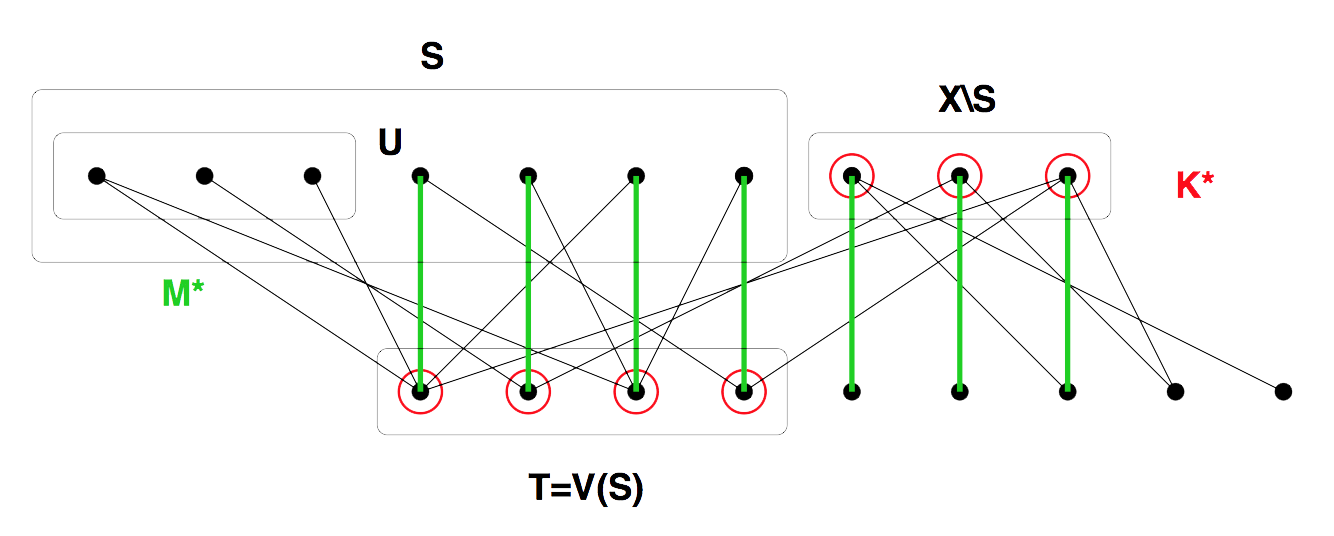
\includegraphics[width=300pt]{../img/konig}
    \end{center}
    Soit $K = T \cup (X \textbackslash S)$, $K$ est une couverture de sommets : toutes les arêtes ont une extrêmité dans $K$ car si ce n'est pas le cas, on a une arête du graphe liant $(Y \textbackslash T)$ à $S$, or $V(S) = T$ (contradictoire). On va montrer que $K$ est une couverture minimale et qu'elle vérifie $|K^*| = |M^*|$.\\
    $|K| = |X \textbackslash S| + |T|$ ($X$ et $Y$ étant disjoints).\\
    Supposons qu'il existe $x \in X \textbackslash S$ tel que $x$ est adjacent par une arête de $M^*$ à un noeud de $T$, dans ce cas $x \in Z$ et donc $x \in S$ (contradictoire). Donc les arêtes de $M^*$ ont une extrémité dans $T$ ou dans $X \textbackslash S$ mais pas dans les deux, donc $|K| = |M^*|$, on a donc trouvé que $K^*$ est une couverture minimum telle que $|K^*| = |M^*|$.\\
    Notons qu'on a pas seulement montré qu'il existe une couverture minimum $K^*$ telle que $|K^*| = |M^*|$, on a aussi vu comment on pouvait la construire connaissant $M^*$.
  \end{proof}
\end{mytheo}

\begin{myexem}[Problème du site de rencontres]
	Nous avons 5 filles et 5 garçons (noeuds) et nous devons en accoupler un maximum en fonction de leurs préférences (arêtes = volonté de s'accoupler). Par conséquent, nous devons réaliser un couplage maximum sur un graphe biparti. Voici le schéma obtenu :
	\begin{center}
	  \begin{tikzpicture}
      \node[vertex] at (-2, 2) (a) {A};
			\node[vertex] at (-1, 2) (b) {B};
			\node[vertex, fill = red] at (0, 2) (c) {C};
			\node[vertex, fill = red] at (1, 2) (d) {D};
			\node[vertex] at (2, 2) (e) {E};
			\node[vertex] at (-2, -2) (f) {a};
			\node[vertex, fill = red] at (-1, -2) (g) {b};
			\node[vertex] at (0, -2) (h) {c};
			\node[vertex, fill = red] at (1, -2) (i) {d};
			\node[vertex] at (2, -2) (j) {e};

      \draw[red] (a) edge node {} (g);
			\draw[] (a) edge node {} (i);
			\draw[] (b) edge node {} (g);
			\draw[] (c) edge node {} (f);
			\draw[] (c) edge node {} (g);
			\draw[red] (c) edge node {} (h);
			\draw[] (c) edge node {} (i);
			\draw[] (c) edge node {} (j);
			\draw[] (d) edge node {} (h);
			\draw[red] (d) edge node {} (j);
			\draw[red] (e) edge node {} (i);
  	\end{tikzpicture}
  \end{center}
On voit que $|M|=|K|$ et, par conséquent (voir en rouge), le couplage est maximum (et la couverture est minimum).
\end{myexem}

\subsection{L'algorithme hongrois}
\index{algorithme!algorithme hongrois}
\begin{myalgo}[Algorithme hongrois venant du cours de R. Lambiotte et L. Tabourier (FUNDP)]
  \noindent
  \begin{enumerate}
    \item Construire un couplage $M$ du graphe biparti tel qu'on ne puisse plus ajouter d'arêtes sans que deux arêtes soient incidentes au même noeud
    \item Soit $U = \{u \in X$ et $u$ non-incident à $M^*\}$, si $U = \o$, le couplage est maximum (arrêt)
    \item $\forall u \in U$, on construit l'ensemble des chemins M-alternés partant de $u$ (étape non-triviale)
      \begin{itemize}
        \item soit aucun de ces chemins n'est M-augmenté, par théorème le couplage est maximum (arrêt)
        \item soit il existe un chemin M-augmenté $u,y_a,x_b,...,x_l,y_m$, et on modifie M selon :\\
        $M \leftarrow M \textbackslash\{(y_a,x_b),...,(y_k,x_l)\} \cup \{(u,ya),(xb,yc),...,(xl,ym)\}$
      \end{itemize}
    \item on itère le procédé jusqu'à avoir un couplage maximum
  \end{enumerate}
\end{myalgo}
\begin{myexem}
  \noindent
  \begin{enumerate}
    \item couplage initial :\\
      \begin{center}
        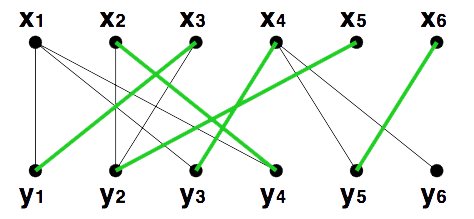
\includegraphics[width=150pt]{../img/hongrois1}
      \end{center}
    \item recherche des chemins alternés :\\
      \begin{center}
        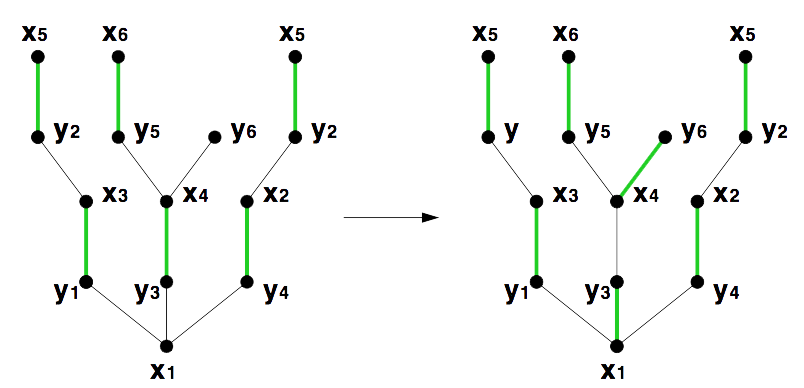
\includegraphics[width=250pt]{../img/hongrois2}
      \end{center}
    \item couplage suivant (et maximum) :\\
      \begin{center}
        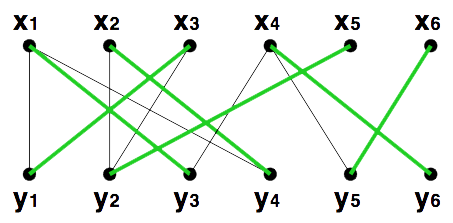
\includegraphics[width=150pt]{../img/hongrois3}
      \end{center}
  \end{enumerate}
\end{myexem}

\section{Coloriages d'arêtes}
\subsection{Coloriages d'arêtes}
%il manque encore qq définitions

%dessin d'un graphe avec professeur et classes
\paragraph{Problème des horaires}
Chaque professeur doit enseigner à un certain nombre de classes pendant un certain nombre d'heures. On veut créer
un horaire sur le plus petit nombre de période possible
\\On relie chaque professeur aux classes auxquelles il donne cours en veillant a colorier les arêtes en fonction des tranches horaires. Deux arêtes de la même couleur ne peuvent pas partir du même nœud.

\index{coloriage}
\index{coloriage!coloriage d'arêtes}
\index{coloriage!coloriage d'arêtes propre}
\begin{mydef}
  Un \emph{coloriage} des arêtes d’un graphe en $k$ couleurs est l’assignation à chaque arête d’une couleur $1, 2, \ldots,$ ou $k$.
  Ce coloriage est dit \emph{propre} si deux arêtes adjacentes sont toujours de couleurs différentes.
\end{mydef}

\index{chromatique!indice chromatique}
\begin{mydef}
  L’\emph{indice chromatique} d’un graphe $G$, noté $\chi '$ ($G$) est le nombre minimal de couleurs nécessaire pour obtenir un coloriage propre des arêtes de $G$.
\end{mydef}


\begin{mytheo}[König]
  Pour tout graphe biparti: $\chi '= \degmax$
  \begin{proof}
    On va utiliser le corrolaire~\ref{corr:hall} du théorème~\ref{theo:hall} de Hall
    pour les graphes bipartis réguliers (qui ont toujours un couplage parfait).
    \begin{enumerate}
      \item Soit un graphe biparti $k$-régulier. Par le théorème de Hall, il existe un couplage parfait. On le colorie en couleur $c_{1}$. On considère ensuite les arêtes restantes non encore coloriées: elles forment un graphe $k-1$ régulier. On recommence pour la couleur $c_{2}$ avec un autre couplage. On continue jusqu'à épuisement, on obtient alors $\chi '=k$
      \item Pour un graphe biparti quelconque de degré maximum $k$.
        \begin{itemize}
          \item Ajouter des nœuds d'un côté si nécessaire pour avoir le même nombre de nœuds de chaque côté.
          \item Si tous les nœuds ne sont pas de degré $k$, alors il y a au moins 1 nœuds de degré $<k$ de chaque côté.
            On ajoute alors une arête entre eux. On recommence jusqu'à $k$-régularité.
        \end{itemize}
        Par le point 1. , il existe un coloriage propre à $k$ couleurs. On supprime ensuite les arêtes et nœuds ajoutés: on obtient un coloriage propre pour le graphe de départ.
        $$\Rightarrow \degmax \le \chi ' \le k = \degmax$$
        $$\Rightarrow \chi ' = k$$
    \end{enumerate}
  \end{proof}
\end{mytheo}

\begin{mytheo} [Vizing]
Pour tout graphe simple: $\chi ' = \degmax$ ou  $\chi ' = \degmax + 1$
  \begin{proof} On sait que $\chi' \ge \degmax$, il faut donc prouver que $\chi ' \le \degmax + 1$.
  \\On le prouve par induction sur le nombre d'arêtes du graphe.
  \\ \textbf{Pas inductif:} Vrai pour $m$ arêtes. Soit un graphe à  $m+1$ arêtes, de degré max $k$. Je retire une de ces arêtes: il existe un coloriage propre à $\le k+1$ couleurs.
  \begin{itemize}
  \item Si $\le k$ couleurs: je choisis (k+1) couleurs pour la $(m+1)^{ième}$ arête.
  \item Si $k+1$ couleurs $c_{1},...,c_{k+1}$: je rétablis la $(m+1)^{ième}$ arête: il faut trouver une couleur pour cette arête.
  \end{itemize}

  \end{proof}
\end{mytheo}
\textbf{Observation:} En chaque nœud il y a au moins une couleur libre (c'est à dire pas utilisée par les arêtes incidentes)
\\
\newline Voici 3 exemples avec $k=3$ et 4 couleurs \emph{noir, bleu, rouge et vert}
\begin{myexem} \label{exemple1}
  Même couleur libre \emph{rouge} pour $x$ et $y$ $\Rightarrow$ on peut utiliser le \emph{rouge} pour $xy$
  \begin{figure}[H]
    \begin{center}
      \subfigure[]{
        \begin{tikzpicture}[scale = 1]
          \draw[thick,black] (0,1) -- (2,1.5);
          \draw[thick,blue] (0,1) -- (2,0.5);
          \draw[thick,dotted,black] (0,1) -- (0,-1);
          \draw[thick,black] (0,-1) -- (2,-0.5);
          \draw[thick,blue] (0,-1) -- (2,-1.5);

          \node at (-0.25,1) {$x$};
          \node at (-0.25,-1){$y$};
        \end{tikzpicture}
      }
      \subfigure[]{
        \begin{tikzpicture}[scale = 1]
          \draw[thick,black] (0,1) -- (2,1.5);
          \draw[thick,blue] (0,1) -- (2,0.5);
          \draw[very thick,red] (0,1) -- (0,-1);
          \draw[thick,black] (0,-1) -- (2,-0.5);
          \draw[thick,blue] (0,-1) -- (2,-1.5);

          \node at (-0.25,1) {$x$};
          \node at (-0.25,-1){$y$};
        \end{tikzpicture}
      }
    \end{center}
  \end{figure}
\end{myexem}

\begin{myexem}
  Pas de couleur libre entre $x$ et $y$. Mais le \emph{noir} est libre pour $y$\\
  $\Rightarrow$ on utilise le \emph{noir} pour $xy$, on efface l'arête \emph{noir} $xy'$\\
  $\Rightarrow$ On se retrouve dans le cas \ref{exemple1}, on utilise ensuite la couleur \emph{vert} pour $xy'$\\
  \begin{figure}[H]
    \begin{center}
      \subfigure[]{
        \begin{tikzpicture}[scale = 1]
          \draw[thick,red] (0,1) -- (2,1.5);
          \draw[thick,green] (0,1) -- (2,0.5);
          \draw[thick,dotted,black] (0,1) -- (0,-1);
          \draw[thick,black] (0,-1) -- (2,-0.5);
          \draw[thick,blue] (0,-1) -- (2,-1.5);
          \draw[thick,blue] (2,-0.5) -- (4,0);
          \draw[thick,red] (2,-0.5) -- (4,-1);

          \node at (-0.25,1) {$y$};
          \node at (-0.25,-1){$x$};
          \node at (1.90,-0.25){$y'$};
        \end{tikzpicture}
      }
      \subfigure[]{
        \begin{tikzpicture}[scale = 1]
          \draw[thick,red] (0,1) -- (2,1.5);
          \draw[thick,green] (0,1) -- (2,0.5);
          \draw[very thick,black] (0,1) -- (0,-1);
          \draw[thick,dotted,black] (0,-1) -- (2,-0.5);
          \draw[thick,blue] (0,-1) -- (2,-1.5);
          \draw[thick,blue] (2,-0.5) -- (4,0);
          \draw[thick,red] (2,-0.5) -- (4,-1);

          \node at (-0.25,1) {$y$};
          \node at (-0.25,-1){$x$};
          \node at (1.90,-0.25){$y'$};
        \end{tikzpicture}
      }
    \end{center}
  \end{figure}
\end{myexem}

\begin{myexem}
  Quelques fois cette astuce ne suffit pas:\\
  \begin{figure}[H]
    \begin{center}
	    \begin{tikzpicture}[scale = 1]
        \draw[thick,red] (0,1) -- (2,1.5);
        \draw[thick,green] (0,1) -- (2,0.5);
        \draw[thick,dotted,black] (0,1) -- (0,-1);
        \draw[thick,black] (0,-1) -- (2,-0.5);
        \draw[thick,blue] (0,-1) -- (2,-1.5);
        \draw[thick,green] (2,-0.5) -- (4,-0.25);
        \draw[thick,red] (2,-0.5) -- (4,-0.75);
        \draw[thick,red] (2,-1.5) -- (4,-1.25);
        \draw[thick,green] (2,-1.5) -- (4,-1.75);
        \draw[thick,black] (4,-0.75) -- (6,-0.5);
        \draw[thick,black] (4,-1.25) -- (6,-1.5);
        \draw[thick,red] (6,-0.5) -- (6,-1.5);

        \node at (-0.25,1) {$y$};
        \node at (-0.25,-1){$x$};
        \node at (1.90,-0.25){$y'$};
        \node at (1.90,-1.78){$y''$};
      \end{tikzpicture}
    \end{center}
  \end{figure}
  Échangeons le \emph{noir} et \emph{rouge} le long du chemin des arêtes de couleurs \emph{noir} et \emph{vert} issus de $xy'$ (le coloriage reste propre) :\\
  \begin{figure}[H]
    \begin{center}
      \begin{tikzpicture}[scale = 1]
        \draw[thick,red] (0,1) -- (2,1.5);
        \draw[thick,green] (0,1) -- (2,0.5);
        \draw[thick,dotted,black] (0,1) -- (0,-1);
        \draw[thick,red] (0,-1) -- (2,-0.5);
        \draw[thick,blue] (0,-1) -- (2,-1.5);
        \draw[thick,green] (2,-0.5) -- (4,-0.25);
        \draw[thick,black] (2,-0.5) -- (4,-0.75);
        \draw[thick,black] (2,-1.5) -- (4,-1.25);
        \draw[thick,green] (2,-1.5) -- (4,-1.75);
        \draw[thick,red] (4,-0.75) -- (6,-0.5);
        \draw[thick,red] (4,-1.25) -- (6,-1.5);
        \draw[thick,black] (6,-0.5) -- (6,-1.5);

        \node at (-0.25,1) {$y$};
        \node at (-0.25,-1){$x$};
        \node at (1.90,-0.25){$y'$};
        \node at (1.90,-1.78){$y''$};
      \end{tikzpicture}
    \end{center}
  \end{figure}
  $c_{1}$ libre $\Rightarrow$ même cas que: \ref{exemple1}
\end{myexem}

% FIXME L'argument ne suffit pas, il faut considérer le cas y'' = y !!

\section{Cliques, ensembles indépendants et l'impossible désordre}

\subsection{Ensembles indépendants}

\begin{mytheo} [Théorème de l'amitié 1] \label{ami1}
  Parmi six personnes, on en trouve toujours trois qui se connaissent l'une l'autre, ou trois qui sont étrangers l'un à l'autre.
  \begin{proof}
     Considérons le graphe complet $K_6$ pour représenter le problème.
     Les nœuds symbolisent les personnes et les arêtes symbolisent les relations entre elles.
     Deux personnes sont reliées par une arêtes bleue si elles se connaissent, et par une arête rouge sinon.
     On veut montrer que le graphe contient un triangle bleu ou un triangle rouge.

     Chaque nœud $x$ a cinq voisins. On peut donc définir une couleur majoritaire en chaque nœud comme la couleur du plus grand nombre d'arêtes incidentes. Prenons le cas où la couleur majoritaire pour $x$ est le bleu. Il existe donc au moins trois arêtes bleues incidentes à $x$.

   \begin{figure} [!h]
   \centering
        \begin{tikzpicture}[scale = 0.5]
                   \draw[blue] (0,1) -- (-1,-1);
                   \draw[blue] (0,1) -- (0,-1.5);
                   \draw[blue] (0,1) -- (1,-1);
                   \draw[black] (0,1) -- (2,0.5);
                   \draw[black] (0,1) -- (2,1.5);

                   \fill[black] (0,1) circle (0.2cm);
                   \fill[black] (-1,-1) circle (0.1cm);
                   \fill[black] (0,-1.5) circle (0.1cm);
                   \fill[black] (1,-1) circle (0.1cm);
                   \fill[black] (2,0.5) circle (0.1cm);
                   \fill[black] (2,1.5) circle (0.1cm);

                   \node at (0,1.5) {$x$};
                   \node at (-1.5,-1.5) {$a$};
                   \node at (0.5,-2) {$b$};
                   \node at (1.5,-1) {$c$};

        \end{tikzpicture}
	\end{figure}

     Considérons trois nœuds $a$, $b$ et $c$ reliés à $x$ par une arête bleue.
     Si ces trois nœuds forment un triangle rouge, alors le graphe contient un triangle rouge.
     Sinon, le triangle $abc$ contient au moins une arête bleue.
     Prenons par exemple l'arête $ab$ bleue. Le triangle $abx$ est alors bleu.
     Le graphe contient donc dans ce cas-ci un triangle bleu.

     La preuve reste évidemment valable si l'on prend l'arête $bc$ ou l'arête $ac$ bleue,
     de même que si l'on prend le rouge comme couleur majoritaire du nœud $x$.
  \end{proof}
\end{mytheo}

\begin{mytheo} [Théorème de l'amitié 2] \label{ami2}
  En coloriant, de façon arbitraire, les arêtes du graphe complet à six nœuds en bleu et rouge, on crée un triangle bleu ou un triangle rouge.
  \begin{proof}
  	Voir théorème \ref{ami1}.
  \end{proof}
\end{mytheo}

\index{ensemble indépendant}
\begin{mydef}
  Un \emph{ensemble indépendant} d'un graphe est un ensemble de nœuds deux à deux non adjacents.
\end{mydef}

\index{ensemble indépendant!maximum}
\begin{mydef}
  Un \emph{ensemble indépendant maximum} est un ensemble indépendant dont le nombre de nœuds est maximal.
\end{mydef}

\begin{mytheo}
Un ensemble de nœuds est indépendant si et seulement si son complémentaire est une couverture de sommets.
\begin{proof}
Soit $S$ un ensemble de nœuds indépendant.

$S$ est un ensemble de nœuds indépendant.
\begin{itemize}
  \item[$\Leftrightarrow$] Il n'existe pas d'arête rejoignant 2 nœuds de $S$.
  \item[$\Leftrightarrow$] Toute arête a au moins une extrémité qui n'est pas incluse dans $S$.
  \item[$\Leftrightarrow$] Le complémentaire de $S$ est une couverture de sommets.
\end{itemize}
\end{proof}
\end{mytheo}

\begin{myexem} \label{cm7:ex1}
	Complémentaire d'un ensemble indépendant
	\begin{figure} [!h]
	\centering
         \begin{tikzpicture}[scale = 0.5]
             	   \draw (-1,0) -- (-2,2) -- (0,3.5) -- (2,2) -- (1,0) -- (-1,0) -- cycle;
                   \draw (-1,0) -- (0,1.5);
                   \draw (-2,2) -- (0,1.5);
                   \draw (0,3.5) -- (0,1.5);
                   \draw (2,2) -- (0,1.5);
                   \draw (1,0) -- (0,1.5);

                   \fill[red] (-1,0) circle (0.2cm);
                   \fill[green] (-2,2) circle (0.2cm);
                   \fill[green] (0,3.5) circle (0.2cm);
                   \fill[red] (2,2) circle (0.2cm);
                   \fill[green] (1,0) circle (0.2cm);
                   \fill[green] (0,1.5) circle (0.2cm);

        \end{tikzpicture}
	\end{figure} \newline
	\color{green}Couverture de sommets \\
	\color{red}Ensemble indépendant (maximal)
	\color{black}
\end{myexem}


\begin{mycorr}
|ensemble indépendant maximum| + |couverture minimum| = |nombre de nœuds|
\end{mycorr}

Ainsi, trouver un ensemble indépendant maximum est tout aussi difficile que de trouver une couverture de sommets minimale.

\subsection{Cliques}

\begin{mydef}
Une \emph{clique} d'un graphe est un ensemble de nœuds deux à deux adjacents. Autrement dit, c'est un sous-graphe complet.
\end{mydef}

\index{clique!maximum}
\begin{mydef}
Une \emph{clique maximum} est une clique dont le nombre de nœuds est maximal.
\end{mydef}

\begin{mytheo}
  Un ensemble est indépendant dans un graphe simple si et seulement s'il est une clique dans le graphe complémentaire.
  \begin{proof}
     Soit $S$ un ensemble indépendant dans un graphe simple $G$.

     $S$ est un ensemble indépendant de $G$
     \begin{itemize}
       \item[$\Leftrightarrow$] Deux nœuds quelconques de $S$ sont non-adjacents dans $G$.
       \item[$\Leftrightarrow$] Deux nœuds quelconques de $S$ sont adjacents dans le complémentaire de $G$.
       \item[$\Leftrightarrow$] $S$ est une clique dans le complémentaire de $G$.
     \end{itemize}
  \end{proof}
\end{mytheo}


\begin{myexem} Complémentaire du graphe de l'exemple \ref{cm7:ex1}
	\begin{figure} [!h]
	\centering
             \begin{tikzpicture}[scale = 0.5]
                   \draw (-1,0) -- (0,3.5) -- (1,0) -- (-2,2) -- (2,2) -- (-1,0) -- cycle;

                   \fill[red]   (-1,0)  circle (0.2cm);
                   \fill[black] (-2,2)  circle (0.2cm);
                   \fill[black] (0,3.5) circle (0.2cm);
                   \fill[red]   (2,2)   circle (0.2cm);
                   \fill[black] (1,0)   circle (0.2cm);
                   %\fill[black] (0,1.5) circle (0.2cm);
        \end{tikzpicture}
    \end{figure} \newline
    \color{red}Clique (maximum) \color{black}
\end{myexem}

\begin{mytheo} [Théorème de l'amitié 3]
  Tout graphe simple à six nœuds contient une clique de trois nœuds ou un ensemble indépendant de trois nœuds.
  \begin{proof}
     Soit $G$ un graphe simple. Si l'on colorie toutes les arêtes de $G$ en bleu et que l'on relie tous les nœuds non-adjacents de $G$ avec des arêtes rouges, par le théorème \ref{ami2}, il existe un triangle bleu ou un triangle rouge.
     On a donc montré qu'il existe une clique de trois nœuds (triangle bleu) ou un ensemble indépendant de trois nœuds (triangle rouge).
  \end{proof}
\end{mytheo}


\begin{mydef} [Nombre de Ramsey]
Le \emph{nombre de Ramsey} $R(n_1 , ..., n_k)$ est le plus petit naturel $r$ tel que tout coloriage du graphe complet de $r$ nœuds en $k$ couleurs $c_1, \ldots, c_k$ crée une clique de $n_1$ nœuds de couleur $c_1$, ou une clique de $n_2$ nœuds de couleur $c_2, ...,$ ou une clique de $n_k$ nœuds de couleur $c_k$.
\end{mydef}

\begin{mytheo} [Théorème de Ramsey]
  Le nombre de Ramsey $R(n_1,...,n_k)$ existe.
  \begin{proof}
    Prouvons le par récurrence sur $k$
    \begin{description}
      \item[Initialisation]
        C'est trivial pour $k = 1$ car il n'y a qu'une seule couleur donc $R(n_1) = n_1$.
        C'est vrai pour $k = 2$ par double récurrence sur $n$ et $m$ par the théorème~\ref{theo:erdosszekeres}.
      \item[Induction]
        Supposons que ce soit vrai pour $k$.
        Soit une suite $n_1, n_2, \ldots, n_{k+1}$, on sait que c'est vrai pour 2 et $k$ donc,
        $R(n_k, n_{k+1})$ existe et $R(n_1, \ldots, R(n_k, n_{k+1}))$ existe.
        Dès lors, par le théorème~\ref{theo:kkp1},
        $R(n_1, \ldots, n_k, n_{k+1})$ existe.
    \end{description}
  \end{proof}
\end{mytheo}

\begin{mytheo} [Théorème de Erdös et Szekeres]
  \label{theo:erdosszekeres}
  Pour $m, n \geq 2: R(m, n) \leq R(m, n-1) + R(m-1, n)$.
  \begin{proof}
     Prenons un noeud quelconque $u$ dans un graphe complet à $R(m,n-1) + R(m-1,n)$ noeuds
     avec des arêtes coloriées en bleu ou en rouge. Soit $M$ et $N$ définis tels que
     \begin{align*}
       M & = \{\text{voisins de }u\text{ reliés par des arêtes bleues}\}\\
       N & = \{\text{voisins de }u\text{ reliés par des arêtes rouges}\}.
     \end{align*}

\begin{figure} [!h]
\centering
        \begin{tikzpicture}[scale = 0.5]
                   \draw[blue] (-1,-2) -- (-3,2);
                   \draw[blue] (-1,-2) -- (-2,2);
                   \draw[blue] (-1,-2) -- (-1,2);
                   \draw[blue] (-1,-2) -- (0,2);
                   \draw[blue] (-1,-2) -- (1,2);
                   \draw[red] (-1,-2) -- (3,0);
                   \draw[red] (-1,-2) -- (3,-1);
                   \draw[red] (-1,-2) -- (3,-2);
                   \draw[red] (-1,-2) -- (3,-3);

                   \fill[black] (-1,-2) circle (0.2cm);
                   \fill[black] (-3,2) circle (0.1cm);
                   \fill[black] (-2,2) circle (0.1cm);
                   \fill[black] (-1,2) circle (0.1cm);
                   \fill[black] (-0,2) circle (0.1cm);
                   \fill[black] ( 1,2) circle (0.1cm);
                   \fill[black] (3, 0) circle (0.1cm);
                   \fill[black] (3,-1) circle (0.1cm);
                   \fill[black] (3,-2) circle (0.1cm);
                   \fill[black] (3,-3) circle (0.1cm);

                   \node at (-1.5,-2.5) {$u$};
                   \node at (-3,3.5) {\color{blue}$M$};
                   \node at (4,0.5) {\color{red}$N$};

                   \draw[blue] (-1,2) ellipse (3cm and 1cm);
                   \draw[red]  (3,-1.5) ellipse (1cm and 2cm);
        \end{tikzpicture}
\end{figure}

 On a (simplement la somme des nœuds) que
 $$|M|+|N|+1 = R(m,n-1) + R(m-1,n).$$

 Donc on a que
 \begin{equation} \label{cm7:RM}
   |M| \geq R(m-1,n)
 \end{equation}
 ou bien
 \begin{equation} \label{cm7:RN}
   |N| \geq R(m,n-1)
 \end{equation}

Si on est dans le cas de figure de l'inégalité \ref{cm7:RM}, il y a deux possibilités.
Soit il existe une clique rouge de $n$ nœuds dans $M$ ce qui implique qu'il existe une clique rouge de $n$ nœuds dans le graphe.
Soit il existe une clique bleue de $m-1$ nœuds dans $M$ ce qui en incluant $u$ fait une clique bleue de $m$ nœuds dans le graphe.

Si on est dans le cas de figure de l'inégalité \ref{cm7:RN}, idem mutatis mutandis.
  \end{proof}
\end{mytheo}

\begin{mycorr}
  $R(m,n) \leq \begin{pmatrix}
m+n-2\\
m-1
\end{pmatrix}$.
\end{mycorr}

\begin{mytheo}
  \label{theo:kkp1}
$R(n_1,...,n_k) \leq R \left( n_1,...,n_{k-2},R(n_{k-1},n_k) \right)$.

\begin{proof}
  Prenons un graphe complet à $R(n_1, ..., n_{k-2}, R(n_{k-1}, n_k))$ nœuds et leurs arêtes coloriées en $k$ couleurs. Soit $c_i $ la couleur $i$.

  Faisons semblant que $c_{k-1}$ et $c_{k}$ sont une seule couleur.
  Cela implique qu'il n'y a plus que $k-1$ couleurs.
  Il existe donc une clique à $n_1$ nœuds de couleur $c_1$ ou bien une clique à $n_2$ nœuds de couleur $c_2$ et ainsi de suite jusqu'à la possibilité d'une clique de $R(n_{k-1}, n_k)$ nœuds de couleur $c_{k-1}$ ou $c_{k}$.

  Or par définition de $R(n_{k-1}, n_k)$, cette dernière possibilité revient à dire qu'il existe une clique de $n_{k-1}$ nœuds de couleur $c_{k-1}$ ou une clique de $n_{k}$ nœuds de couleur $c_{k}$.
\end{proof}
\end{mytheo}

\vspace{0.3cm}
En d'autre termes, ce théorème stipule qu'il existe toujours un peu d'ordre dans un ensemble suffisamment grand.

\begin{mytheo} [Théorème de l'amitié 4]
  $R(3, 3) = 6$
  \begin{proof}
     Cela découle directement du théorème \ref{ami2}.
  \end{proof}
\end{mytheo}


\begin{mytheo}
[Théorème de Turán
\footnote{par la contraposée on obtient la définition de Wikipédia qui nous dit: Tout graphe $G$ ayant $n$ sommets, et ne contenant pas de clique de taille plus grande que $r$ ($ K_{r+1} $) possède au plus $(1-\frac{1}{r})\frac{n^2}{2}$ arêtes}] \label{turan}
Si un graphe simple possède strictement plus de $(1-\frac{1}{r})\frac{n^2}{2}$ arêtes, alors il a une clique de $r+1$ nœuds.
\end{mytheo}

Cette borne est atteinte par le graphe de Turán $T(n,r)$.  Selon wiki un graphe de $T(n,r)$ n'a pas de clique de taille $ r+1$ mais je ne sais pas si il existe un graphe $T(n,r)$ pour tout $r$.


\textbf{Notes :}
\begin{enumerate}
\item
Pendant les séances d'exercices, le tuteur a complété le théorème \ref{turan} en ajoutant ``et il existe un graphe possédant $\left( 1-\dfrac{1}{r} \right) \dfrac{n^2}{2}$ qui ne contient aucune clique de taille $r+1$'' (ce que Wikipédia semble confirmer).
\item
On a  $\left( 1-\dfrac{1}{n} \right) \dfrac{n^2}{2} > \left( 1-\dfrac{1}{n-1} \right) \dfrac{n^2}{2}$ donc si on prend $r=n-1$ alors on aura une clique à $(n-1)+1=n$ nœuds. Or on a bien : $\left( 1-\dfrac{1}{n} \right) \dfrac{n^2}{2} = \dfrac{n(n-1)}{2}$.
\end{enumerate}


\subsection{La théorie de Ramsey}
Beaucoup de théorèmes existent qui imitent le théorème de Ramsey et prouvent quelque chose du genre:
\begin{itemize}
\item
``Dans un machin suffisamment grand, il y a toujours des sous-machins avec une certaine propriété.''
\item
``Dans un grand machin, m\^eme tout-à-fait quelconque, un certain ordre est inévitable.''
\item
``Le désordre complet est impossible.''
\end{itemize}



\begin{mytheo} [Sommes d'entiers]
    Si l'on colorie les nombres de un à quatorze en trois couleurs alors il existe trois nombres (pas forcément distincts) $x$, $y$ et $z$ de m\^eme couleur tels que $x+y=z$.
\end{mytheo}

\begin{myexem}
Séparons les nombres de 1 à 13 en trois couleurs:
\vspace*{0.2cm}

    \begin{tabular}{|c|c|c|c|c|c|c|c|c|c|c|c|c|c|}
        \hline
       couleur1 & 1 &  &  & 4  &  &  &  &  &  & 10 &  &  & 13\\

       \hline
       couleur2 &  & 2 & 3 &  &  &  &  &  &  &  & 11 & 12 &\\

       \hline
       couleur3 &  &  &  &  & 5 & 6 & 7 & 8 & 9 &  &  &  &\\

        \hline
      \end{tabular} \\
      Le 14 ne va nulle part.
\end{myexem}

%\vspace*{0.2cm}

\begin{mytheo} [Théorème de Schur]
Pour chaque $k$, il y a un nombre $r_k$ tel que pour toute partition des nombres $1,2,....,r_k$ en $k$ classes, une de ces classes contient $x$, $y$ et $z$ tels que $x+y=z$. \footnote{dans l'exemple ci-dessus $k = 3$ et $r_k = 14$}
\begin{proof}
Soit $r_k = R(n_1,...,n_k)$ avec $\forall i \in [1 , k], n_i = 3 $.

Colorions les ar\^etes du graphe à $r_k$ nœuds, sachant qu'on a réparti arbitrairement ses nœuds dans les classes $S_1 ,S_2,....,S_k$.

Nous allons les colorier de la manière suivante: l'ar\^ete $ij$ est dans la couleur $c$ si $\mid i-j \mid \in S_c $.\footnote{à priori il n'y a pas de raison particulière pour le choix "couleur $c$ si $\mid i-j \mid \in S_c $" mais ça fonctionne.} Nous utilisons donc $k$ couleurs différentes pour les arêtes.

Par le théorème de Ramsey, il y a un triangle monochrome.
Donc il y a $i$, $j$ et $l$ tels que:
\begin{itemize}
\item
$i < j < l$
\item
$j-i, l-j, l-i$ sont dans le m\^eme classe.
\end{itemize}

On prend alors:\\
$x = j-i$, $y = l-j$ et $z = l-i$\\
$\Rightarrow x+y=z$

\end{proof}
\end{mytheo}


\begin{mytheo} [Théorème d'Esther Klein]
Parmi cinq points arbitraires dans le plan, tels que trois d'entre eux ne sont  jamais alignés, on peut toujours en choisir quatre qui déterminent un quadrilatère convexe.
\end{mytheo}

\begin{mytheo}
Si l'on colorie les nombres de un à neuf en deux couleurs.  Alors il existe une progression arithmétique de longueur trois qui est monochrome.
\end{mytheo}

\begin{mytheo} [Théorème de Van der Waerden]
Pour tout $k$, $l$, il existe un nombre $W(k,l)$ tel que les nombres de 1 à $W(k,l)$, coloriés arbitrairement en $k$ couleurs, contiennent une progression arithmétique monochrome de longueur $l$.
\end{mytheo}

\begin{myexem} Cherchons $W(2,3)$ expérimentalement.

\color{green}1 \color{green}2 \color{red}3 \color{green}4 \color{green}5  \color{red}6 \color{red}7 \color{black}8

On ne sait pas en quelle couleur colorier le huit car si on le met en rouge on crée la suite arithmétique 6, 7, 8, de raison un et en vert la suite 2, 5, 8, de raison 3.
\end{myexem}

\section{Séance 8}

\textbf{Coloriage de sommets et polynôme chromatique}

\paragraph{1. } Quels sont les graphes de nombre chromatique égal à 1? et égal à 2?
\begin{solution}
  \begin{enumerate}
    \item Les graphes de nombre chromatique égal à 1 sont forcément les graphes sans arête car dès qu'il y a une arête, on a besoin d'au moins $2$ couleurs pour colorier le graphe (une pour chaque extrémité).
    \item Les graphes de nombre chromatique égal à 2 sont les graphes bipartis. Démontrons la double implication :
    \begin{itemize}
    \item biparti $\Rightarrow \mathcal{X} = 2 $ puisqu'il suffit de colorier tous les noeuds d'un ensemble dans une couleur et les noeuds de l'autre dans une deuxième couleur
    \item $\mathcal{X} = 2 \Rightarrow$ il n'y a pas de cycle de longueur impaire $\Rightarrow$ le graphe est biparti
     \end{itemize}
  \end{enumerate}
\end{solution}

\paragraph{2. } Trouvez le nombre chromatique du graphe de Pétersen, et du graphe biparti complet $K_{5,3}$.
\begin{solution}
  \begin{enumerate}
    \item Nous savons que $3 \leq \mathcal{X}$ car le graphe n'est pas biparti et il existe effectivement un coloriage à  $3$ couleurs :
    \begin{center}
    	\includegraphics[scale=0.4]{seance8ex2}
     \end{center}
    \item  $\mathcal{X} = 2$ car ce graphe est biparti.
  \end{enumerate}
\end{solution}

\paragraph{3. } Vrai ou faux? \\
\begin{enumerate}[(a)]
  \item Un graphe de degré maximum 3 peut être colorié avec 4 couleurs.
  \item Un graphe de degré maximum 4 peut être colorié avec 4 couleurs.
  \item Si $G$ contient $K_n$ comme sous-graphe, alors son nombre chromatique est supérieur ou égal à $n$.
  \item Si $G$ est de nombre chromatique égal à $n$, alors $G$ contient $K_n$ comme sous-graphe.
\end{enumerate}

\begin{solution}
  \begin{enumerate}
    \item Vrai car $\mathcal{X} \leq$ degré max $+ 1 = 4$. 
    \item  Pas toujours. Le graphe $K_5$ en nécessite $5$ par exemple.
    \item Vrai puisqu'on aura déjà besoin de $5$ pour colorier $K_n$.
    \item Faux. Prenons par exemple le graphe de Péterson. Son nombre chromatique est égal à $3$ sans pour qu'il ne contienne de triangle. En fait, dès qu'on aura un cycle de longueur impaire, on va avoir $n \geq 3 $ sans pour autant que le graphe ne contienne $K_n$.
  \end{enumerate}
\end{solution}

\paragraph{4. } L'algorithme glouton de coloration associé à un graphe $G$ fonctionne comme suit: on parcourt les sommets $v_1,v_2,…,v_n$ de $G$ dans un ordre fixé arbitrairement. Lorsqu'on rencontre le sommet $v_i$, on lui assigne la plus petite couleur qui n'est pas encore utilisée par un de ses voisins.
\begin{enumerate}[(a)]
  \item Montrez que tout graphe $G$ possède une séquence de sommets pour laquelle l'algorithme glouton utilise un nombre minimum de couleurs.
  \item Construisez pour tout $k \geq 1$ un arbre de degré maximum $k$ et une séquence de ses sommets pour laquelle l'algorithme glouton utilise $k+1$ couleurs.
\end{enumerate}

\begin{solution}
  \begin{enumerate}
    \item En partant du graphe colorié, on peut créer une telle séquence en mettant d'abord tous les sommets de couleur $1$, puis tous les sommets de couleur $2$, etc. Le graphe obtenu à l'aide de l'algorithme glouton sera peut-être différent de celui qu'on avait au départ dans le sens où cet algorithme assigne la couleur la plus petite possible donc il se peut par exemple qu'il y a un noeud de couleur $2$ qui devienne de couleur $1$. L'algorithme glouton utilisera cependant bien le nombre minimal de couleurs, ce qui est bien ce qu'on veut!
    \item  Soit $A_1$ un noeud isolé. On peut ensuite créer $A_k$, avec $k \geq 2$, en créant un noeud relié à toutes les structures créées précédemment. La figure  ci-dessous illustre une telle construction.
    \begin{center}
    	\includegraphics[scale=0.6]{seance8ex4}
     \end{center}
  \end{enumerate}
\end{solution}


\paragraph{5. } Pour les deux graphes ci-dessous appliquez l'algorithme de coloration glouton, et trouvez $\chi(G)$.


\begin{figure}[h!]
  \centering
  %\begin{center}
  \subfigure[]{
    \begin{tikzpicture}[-,>=stealth',shorten >=1pt,auto]
      \Vertex[x=0 ,y=0]{1}
      \Vertex[x=1 ,y=1]{2}
      \Vertex[x=2,y=0]{3}
      \Vertex[x=1 ,y=-1]{4}
      \Vertex[x=3 ,y=1]{5}
      \Vertex[x=3 ,y=-1]{6}
      \Vertex[x=4 ,y=0]{7}



      \path[every node/.style={font=\sffamily\small}]
      (1) edge node [left] {} (2)
      edge node [left] {} (5)
      edge node [left] {} (3)
      edge node [left] {} (4)
      edge node [left] {} (6)

      (2) edge node [right] {} (3)
      edge node [right] {} (7)
      edge node [right] {} (5)

      (3) edge node [right] {} (4)
      edge node [left] {} (5)
      edge node [left] {} (6)
      edge node [left] {} (7)

      (4) edge node [right] {} (6)
      edge node [right] {} (7)

      (5) edge node [right] {} (7)

      (6) edge node [right] {} (7);

  \end{tikzpicture} }
  \subfigure[]{
    \begin{tikzpicture}[-,>=stealth',shorten >=1pt,auto]
      \Vertex[x=0 ,y=0]{1}
      \Vertex[x=1 ,y=1]{2}
      \Vertex[x=1,y=0]{3}
      \Vertex[x=1 ,y=-1]{4}
      \Vertex[x=3 ,y=1]{5}
      \Vertex[x=3 ,y=-1]{6}
      \Vertex[x=2 ,y=0]{7}

      \path[every node/.style={font=\sffamily\small}]
      (1) edge node [left] {} (2)
      edge node [left] {} (3)
      edge node [left] {} (4)

      (2) edge node [right] {} (3)
      edge node [right] {} (7)
      edge node [right] {} (5)

      (3) edge node [right] {} (4)
      edge node [left] {} (7)

      (4) edge node [right] {} (6)
      edge node [right] {} (7)

      (5) edge node [right] {} (7)
      edge node [right] {} (6)

      (6) edge node [right] {} (7);

    \end{tikzpicture}
  }

\end{figure}

\begin{solution}
  \begin{enumerate}
    \item 
    \begin{itemize}
    \item noeud 1 $\Rightarrow$ couleur 1
    \item noeud 2 $\Rightarrow$ couleur 2
    \item noeud 3 $\Rightarrow$ couleur 3
    \item noeud 4 $\Rightarrow$ couleur 2
    \item noeud 5 $\Rightarrow$ couleur 4
    \item noeud 6 $\Rightarrow$ couleur 4
    \item noeud 7 $\Rightarrow$ couleur 1
    \end{itemize}
    Comme $K_4$ est inclus dans le graphe, on doit avoir $\mathcal{X} \geq 4$  et donc on a effectivement bien $\mathcal{X} = 4$.
    \item
    \begin{itemize}
    \item noeud 1 $\Rightarrow$ couleur 1
    \item noeud 2 $\Rightarrow$ couleur 2
    \item noeud 3 $\Rightarrow$ couleur 3
    \item noeud 4 $\Rightarrow$ couleur 2
    \item noeud 5 $\Rightarrow$ couleur 1
    \item noeud 6 $\Rightarrow$ couleur 3
    \item noeud 7 $\Rightarrow$ couleur 4
    \end{itemize}
    Regardons le cycle 23465. Puisqu'il est de longueur impaire, il va falloir 3 couleurs pour le colorier. Ensuite, on aura besoin d'une autre couleur pour le noeud $7$ comme il est relié à tous les noeuds du cycle. Dès lors, on a effectivement bien $\mathcal{X} = 4$ .
     \end{enumerate}
\end{solution}

\paragraph{6. } Sous quelle condition la somme des coefficients d'un polynôme chromatique est-elle nulle?
\begin{solution}
  La somme des coefficients du polynôme $= \pi_G(1)$ et $\pi_G(1) = 0$ veut dire que G a au moins une arête.
\end{solution}

\paragraph{7. } Trouvez le polynôme chromatique du graphe biparti complet $K_{2,2}$, et donnez le nombre de colorations possibles du cycle $C_4$ avec 5 couleurs.
\begin{solution}
  \begin{enumerate}
  \item En utilisant le fait que $\pi_k(G) = \pi_k(G-e) - \pi_k(G.e)$, on trouve que $\pi_k(K_{2,2}) = k^2(k-1)^2 - k (k-1)^2 - k(k-1)(k-2) = k^4-4k^3+6k^2-3k$.
  \item $C_4$ et $K_{2,2}$ sont isomorphes donc ils ont le même polynôme chromatique et $\pi_5(C_4) = \pi_5(K_{2,2}) = 5^4 - 4\cdot 5^3 + 6\cdot 5^2 - 3\cdot 5 = 260$.
\end{enumerate}
\end{solution}

\paragraph{8. }
\begin{enumerate}[(a)]
  \item Trouvez le polynôme chromatique d'un graphe chemin de longueur $n$
  \item Utilisez ce résultat pour trouver le polynôme chromatique d'un graphe circuit de longueur $n$.
\end{enumerate}
\begin{solution}
  \begin{enumerate}
  \item On démontre par récurrence que $p_k(P_n) = k(k-1)^n$.
  \item Etant donné que $\pi_k(G) = \pi_k(G-e) - \pi_k(G.e)$, on peut écrire que
           \begin{eqnarray*}
           p_k(C_n) &=& p_k(P_{n-1}) - p_k(C_{n-1})\\
           		    &=& k(k-1)^{n-1} - k(k-1)^{n-2} + ... + k(k-1)\\
		             &=& k(k-1) [(k-1)^{n-2} - (k-1)^{n-3} + ... + (-1)^n]\\
		             &=& k(k-1)\frac{1}{k}[(k-1)^{n-1}+(-1)^n]\\
		             &=& (k-1)^n + (-1)^n (k-1)
	   \end{eqnarray*}             
\end{enumerate}
\end{solution}

\paragraph{9. } Soit le graphe parallélépipède $3 \times 3 \times 2$.

\begin{enumerate}[(a)]
  \item Chaque arête du graphe est de longueur 1. On souhaite décrire un chemin qui part du sommet $s$ et arrive au sommet $t$ en passant au moins une fois par chaque arête. Quelle est la longueur minimale d'un tel chemin?
  \item Quel est le nombre minimum de couleurs nécessaires pour colorier les sommets de façon à ce que deux sommets adjacents soient toujours de couleurs différentes?
  \item Soit $P_G(k)$ le polynôme chromatique de ce graphe. Quel est le degré de $P_G(k)$? Que vaut $P_G(2)$?
  \item Trouvez une expression aussi explicite que possible pour le nombre de chemins de longueur $k$ du sommet $s$ à lui-même.
\end{enumerate}

\begin{figure}[h!]
  \centering
  %\includegraphics[scale=0.7]{img_tp8.jpg}
\end{figure}

\section{Graphes planaires}
Un graphe est planaire si il possède une représentation dans le plan dont les arêtes ne se touchent pas, sauf à leurs extrémités.\\

\begin{mytheo}[Conjoncture des quatre couleurs]
Quatre couleurs suffisent toujours pour colorier une carte
\begin{proof}
On suppose qu'en chaque point se rencontrent au maximum trois pays, et que les pays sont d'un seul tenant.\\

\begin{center}
\begin{tikzpicture}
%Outer box
\draw[fill=red] (-3,-3)--(-3,11)--(11,11)--(11,-3)--cycle;
%Outer circle
\draw (0,0) to[out=135,in=-135] (0,8);
\draw (0,8) to[out=45,in=135] (8,8);
\draw (8,8) to[out=-45,in=45] (8,0);
\draw (8,0) to[out=-135,in=-45] (0,0);

%First inner circle
\draw (1,4) to[out=90,in=-135] (2,6);
\draw (2,6) to[out=45,in=-180] (4,7);
\draw (4,7) to[out=0,in=135] (6,6);
\draw (6,6) to[out=-45,in=90] (7,4);
\draw (7,4) to[out=-90,in=45] (6,2);
\draw (6,2) to[out=-135,in=0] (4,1);
\draw (4,1) to[out=-180,in=-45] (2,2);
\draw (2,2) to[out=135,in=-90] (1,4);

%Second inner circle
\draw (3,4) to[out=90,in=-180] (4,5);
\draw (4,5) to[out=0,in=90] (5,4);
\draw (5,4) to[out=-90,in=0] (4,3);
\draw (4,3) to[out=-180,in=-90] (3,4);

%Links from Outer to first inner
\draw (0,0)--(2,2);
\draw (0,8)--(2,6);
\draw (8,8)--(6,6);
\draw (8,0)--(6,2);

%Links from first inner to second
\draw (1,4)--(3,4);
\draw (4,7)--(4,5);
\draw (7,4)--(5,4);
\draw (4,1)--(4,3);

%Regions
%1
\draw [fill = green](2,6) to[out=45,in=-180](4,7)to[out=0,in=135] (6,6)--(8,8)to[out=135,in=45](0,8)--(2,6);
\draw [fill= green](3,4) to[out=90,in=-180] (4,5)to[out=0,in=90](5,4) to[out=-90,in=0] (4,3)to[out=-180,in=-90] (3,4);
\draw[fill=green] (6,2) to[out=-135,in=0] (4,1)to[out=-180,in=-45] (2,2)--(0,0) to[out=-45,in=-135] (8,0)--(6,2);
%3
\draw [fill=yellow] (4,1) to[out=-180,in=-45] (2,2)to[out=135,in=-90] (1,4)--(3,4)to[out=-90,in=-180] (4,3)--(4,1);
\draw [fill=yellow] (4,7) to[out=0,in=135] (6,6)to[out=-45,in=90] (7,4)--(5,4)to[out=90,in=0] (4,5)--(4,7);
%4
\draw [fill=blue] (2,2) to[out=135,in=-90] (1,4)to[out=90,in=-135] (2,6)--(0,8)to[out=-135,in=135] (0,0)--(2,2);
\draw [fill=blue] (6,6) to[out=-45,in=90] (7,4)to[out=-90,in=45] (6,2)--(8,0)to[out=45,in=-45] (8,8)--(6,6);
\end{tikzpicture}
\end{center}

Il est possible de partir du graphe correspondant en remplacant les pays par des sommets et les frontières par des arêtes. Ce graphe est alors planaire. Il suffit alors de montrer que tout graphe planaire a un nombre chromatique $\chi \leq 4$ (ou de manière équivalente, admet au moins un coloriage de quatre couleurs).\\

\end{proof}
\end{mytheo}

Notons qu'un graphe planaire peut être dessiné de manière non planaire.

\begin{center}

  \begin{tikzpicture}
    \node[fill=black,  circle, inner sep=0pt,minimum width=0.5mm] (test) at (0,0) {\textbullet};
    \node[fill=black,  circle, inner sep=0pt,minimum width=0.5mm] (test) at (0,4) {\textbullet};
    \node[fill=black,  circle, inner sep=0pt,minimum width=0.5mm] (test) at (4,4) {\textbullet};
    \node[fill=black,  circle, inner sep=0pt,minimum width=0.5mm] (test) at (4,0) {\textbullet};
    \node[fill=black,  circle, inner sep=0pt,minimum width=0.5mm] (test) at (2,6) {\textbullet};
    \node[fill=black,  circle, inner sep=0pt,minimum width=0.5mm] (test) at (1,2) {\textbullet};
    \node[fill=black,  circle, inner sep=0pt,minimum width=0.5mm] (test) at (3,2) {\textbullet};

    \draw (0,0)--(0,4)--(2,6)--(4,4)--(4,0)--cycle;
    \draw (0,4)--(4,4);
    \draw (0,0)--(1,2)--(2,6);
    \draw (4,0)--(3,2)--(2,6);
    \draw (0,4) to[out=-89, in=179] (4,0);
  \end{tikzpicture}

  \begin{tikzpicture}
    \node[fill=black,  circle, inner sep=0pt,minimum width=0.5mm] (test) at (1,0) {\textbullet};
    \node[fill=black,  circle, inner sep=0pt,minimum width=0.5mm] (test) at (1,4) {\textbullet};
    \node[fill=black,  circle, inner sep=0pt,minimum width=0.5mm] (test) at (5,4) {\textbullet};
    \node[fill=black,  circle, inner sep=0pt,minimum width=0.5mm] (test) at (5,0) {\textbullet};
    \node[fill=black,  circle, inner sep=0pt,minimum width=0.5mm] (test) at (3,6) {\textbullet};
    \node[fill=black,  circle, inner sep=0pt,minimum width=0.5mm] (test) at (0,2) {\textbullet};
    \node[fill=black,  circle, inner sep=0pt,minimum width=0.5mm] (test) at (6,2) {\textbullet};
    \draw (1,0)--(1,4)--(3,6)--(5,4)--(5,0)--cycle;
    \draw (1,4)--(5,4);
    \draw (1,0) to[out=135,in=-90](0,2)to[out=90,in=-150](3,6);
    \draw (5,0) to[out=45,in=-90](6,2)to[out=90,in=-30](3,6);
    \draw (1,4)--(5,0);
  \end{tikzpicture}
\end{center}





\subsection{Graphes planaires}
\begin{mytheo} [Fáry]
  Tout graphe planaire simple peut être représenté en n'utilisant que des arêtes droites.
  %no proof ?
\end{mytheo}



\begin{mytheo}
Le graphe complet $K_5$ à cinq noeuds n'est pas planaire.

  \begin{proof}

  Représentons $K_5$ dans le plan. Soit l'ensemble de ses noeuds $\{v_1, v_2, v_3, v_4, v_5\}$.\\
  $v_1, v_2$ et $v_3$ forment un triangle. Où placer $v_4$?

    \begin{center}
      \begin{tikzpicture}
        \node[circle] (v1)[draw=black] at (0,0) {$v_1$};
        \node[circle] (v2)[draw=black] at (7,0) {$v_2$};
        \node[circle] (v3)[draw=black] at (2,5) {$v_3$};
        \draw (v1)--(v2)--(v3)--(v1);
      \end{tikzpicture}
    \end{center}


  \begin{enumerate}
    \item A l'intérieur du triangle formé par $v_1, v_2$ et $v_3$ ?\\
    \begin{center}
      \begin{tikzpicture}
        \node[circle] (v1)[draw=black] at (0,0) {$v_1$};
        \node[circle] (v2)[draw=black] at (7,0) {$v_2$};
        \node[circle] (v3)[draw=black] at (2,5) {$v_3$};
        \node[circle] (v4)[draw=black] at (3,2) {$v_4$};
        \draw (v1)--(v2)--(v3)--(v1);
        \draw (v4)--(v1);
        \draw (v4)--(v2);
        \draw (v4)--(v3);
      \end{tikzpicture}
    \end{center}
    %\includegraphics[scale=0.4]{t2}\\
    Où placer $v_5$?
    \begin{enumerate}
      \item A l'intérieur du triangle formé par $v_1, v_3$ et $v_4$ ? Le graphe ne serait plus planaire puisqu'il faudrait couper le triangle $v_1, v_3$ et $v_4$ pour relier $v_5$ à $v_2$.\\
      \begin{center}
        \begin{tikzpicture}
          \node[circle] (v1)[draw=black] at (0,0) {$v_1$};
          \node[circle] (v2)[draw=black] at (7,0) {$v_2$};
          \node[circle] (v3)[draw=black] at (2,5) {$v_3$};
          \node[circle] (v4)[draw=black] at (3,2) {$v_4$};
          \node[circle] (v5)[draw=black] at (1.8,2.2) {$v_5$};
          \draw (v1)--(v2)--(v3)--(v1);
          \draw (v4)--(v1);
          \draw (v4)--(v2);
          \draw (v4)--(v3);
        \end{tikzpicture}
      \end{center}
      %\includegraphics[scale=0.4]{t3}
      \item A l'intérieur de $v_1$, $v_2$, $v_4$ ou de $v_2$, $v_3$, $v_4$ ? Idem.
      \item A l'extérieur de $v_1$, $v_2$, $v_3$? \\
      \begin{center}
        \begin{tikzpicture}
          \node[circle] (v1)[draw=black] at (0,0) {$v_1$};
          \node[circle] (v2)[draw=black] at (7,0) {$v_2$};
          \node[circle] (v3)[draw=black] at (2,5) {$v_3$};
          \node[circle] (v4)[draw=black] at (3,2) {$v_4$};
          \node[circle] (v5)[draw=black] at (0,3) {$v_5$};
          \draw (v1)--(v2)--(v3)--(v1);
          \draw (v4)--(v1);
          \draw (v4)--(v2);
          \draw (v4)--(v3);
        \end{tikzpicture}
      \end{center}
      %\includegraphics[scale=0.4]{t4}\\
    \end{enumerate}
    \item A l'extérieur de $v_1, v_2$, $v_3$ ? En applicant le même type d'énumération qu'au point précédent, on trouve qu'il n'y a aucune manière de représenter $K_5$ dans le plan de manière à ce qu'il soit planaire.
  \end{enumerate}
  \end{proof}
\end{mytheo}



\begin{mytheo}
Le graphe complet biparti $K_{3,3}$ à $3+3$ noeuds n'est pas planaire.
%proof avec Euler après
\end{mytheo}

\index{subdivision}
\begin{mydef}
  Une \emph{subdivision} d'un graphe est un graphe obtenu en remplaçant chaque arête
  par un chemin (possiblement de longueur 1).
\end{mydef}

\begin{mytheo} [Kuratowski]
  Un graphe est non planaire si et seulement s'il contient comme sous-graphe $K_5$ ou $K_{3,3}$ ou une subdivision de ceux-ci.
%pas de preuve
\end{mytheo}

\begin{mytheo}
  Une \emph{subdivision} d'un graphe non planaire est non-planaire,
  et un sous-graphe d'un graphe planaire est planaire.
\end{mytheo}

\index{face}
\index{face!face extérieure}
\index{face!face intérieure}
\begin{mydef}
  Un graphe planaire (dans une représentation sans croisement) découpe le plan en plusieurs régions connexes (au sens géométrique). Ces régions sont appelées \emph{faces}. Il y a une et une seule face non bornée, nommée \emph{face extérieure}, les autres faces sont \emph{intérieures}.
\end{mydef}

\index{face!bord d'une face}
\index{face!face incidente}
\index{face!degré d'une face}
\begin{mydef}
  On identifie le \emph{bord d'une face} au parcours fermé qui longe la face. Le bord parcourt chaque arête une ou deux fois.
  Une face est \emph{incidente} aux arêtes et sommets qui sont sur son bord.
  Le \emph{degré d'une face} est la longueur du bord, donc le nombre d'arêtes incidentes (comptées une ou deux fois).
\end{mydef}

\index{dual}
\begin{mydef}
  Etant donné un graphe planaire $G$ (dans une représentation sans croisement), construisons $G^*$ , graphe dont les sommets sont les faces de $G$, reliés si et seulement si les faces correspondantes ont dans $G$ une arête en commun. Ce graphe $G^*$ est le \emph{dual} de $G$ (dans cette représentation).
\end{mydef}

\begin{myexem}
\noindent
\textit{Exemple} :
  \begin{center}
    \begin{tikzpicture}
    %Premier graphe
    \node[circle](N1)[draw=black] at (4,10) {1};
    \node[circle](N2)[draw=black] at (4,8) {2};
    \node[circle](N3)[draw=black] at (8,5) {3};
    \node[circle](N4)[draw=black] at (4,2) {4};
    \node[circle](N5)[draw=black] at (0,5) {5};
    \node[circle](N6)[draw=black] at (2.5,5){6};

    \draw (N1)--(N2)--(N3)--(N4)--(N5)--(N2);
    \draw (N5)to[out=20,in=160](N6)to[out=-160,in=-20](N5);
    \draw (N6)--(N2);

    %Second graphe
    \node (NN7) at (1.25,5) {\textbullet};
    \node (NN8) at (2.5,6) {\textbullet};
    \node (NN9) at (7,10) {\textbullet};
    \node (NN10) at (6,5) {\textbullet};
    \node [red] (test) at (8,11){Graphe Dual};
    \node [black] (test) at  (7,2){Face extérieure};
    \node [draw,text width =4.5cm] (test) at (12,10)
    {4 faces\\
    Face extérieure : 1234521\\
    degré(face extérieure) = 6};

    \coordinate (N7) at (1.25,5);
    \coordinate (N8) at (2.5,6);
    \coordinate (N9) at (7,10);
    \coordinate (N10) at (6,5);

    \draw[red] (N7) to[out=-20,in=-160](N10)--(N8)--(N7);
    \draw[red] (N10)to[out=-160,in=90](1.5,2)to[out=-90,in=-180](4,0.5)to[out=0,in=-135](11,2.5)to[out=45,in=-30](N9)to[out=130,in=45](2,11)to[out=-135,in=135](N8);
    \draw[red] (N10)to[out=-45,in=-135](8.5,4)to[out=45,in=-30](N9);
    \draw[red] (N10)--(N9);
    \draw[red] (N9) to[out=170,in=90](3,10)to[out=-90,in=-170](N9);

    \end{tikzpicture}
  \end{center}
\end{myexem}


\begin{mytheo}
  La somme des degrés des faces est deux fois le nombre d'arêtes.
  \begin{proof}
    On passe au graphe dual, sur lequel on applique le théorème des poignées de mains.
  \end{proof}
\end{mytheo}

\begin{mytheo}
  Un graphe est planaire si et seulement si il est représentable sur la sphère sans croisement d'arêtes.
  \begin{proof}
  On utilise la projection stéréographique pour passer d'une représentation planaire à une représentation sphérique et vice versa.
  \end{proof}
\end{mytheo}

\subsection{Formule d'Euler}
\begin{mytheo} [Formule d'Euler]
  Dans un graphe planaire connexe à $n$ sommets, $e$ arêtes et $f$ faces:
  $$n − e + f = 2$$
  \begin{proof}
    On démontre cette égalité par récurrence sur le nombre de faces
    \begin{description}
      \item[Initialisation]
        S'il y a une seule face, alors le graphe est sans cycle car chaque cycle créé au moins 2 faces, la face intérieure au cycle
        et la face extérieure au cycle.
        C'est donc un arbre d'où $e = n-1$, c'est à dire $n - e + f = 2$ car $f = 1$.
      \item[Induction]
        Soit un graphe $G$ avec $f > 1$ faces.
        Comme les arbres ont une seule face, $G$ possède un cycle et donc deux faces adjacentes.
        Soit $G'$ obtenu en supprimant une arête entre les deux faces.
        Les deux faces deviennent une seule face pour $G'$.
        Ce graphe a donc $f - 1$ faces et $e-1$ arêtes, par l'hypothèse de récurrence sur $G'$, on a
        \begin{align*}
          n - (e-1) + (f-1) & = 2\\
          n - e + f & = 2.
        \end{align*}
    \end{description}
  \end{proof}
\end{mytheo}

\begin{mytheo}
  \label{theo:threensix}
  Dans tout graphe planaire \emph{simple} à $n \geq 3$ sommets et $e$ arêtes,
  $e \leq 3n - 6$.
  \begin{proof}
    Commençons par montrer que pour toute face $f$, $\deg(f) \geq 3$.
    Pour la face extérieure, c'est vrai car $n \geq 3$.
    Pour une face intérieure, comme le graphe est simple, la plus petite face en terme de degré est un triangle donc c'est vrai également.

    On a donc
    \[ \sum_{f \in F} \deg(f) \geq 3 |F|. \]
    Or par le théorème des poignées de main dual,
    \[ \sum_{f \in F} \deg(f) = 2 |E|. \]
    Et donc
    \begin{equation} \label{ineg6}
      \frac{2}{3} e \geq |F|.
    \end{equation}
    En injectant \ref{ineg6} dans la formule d'Euler, on obtient
    \[ 2 = n - e + |F| \leq n - e + \frac{2}{3}e \]
    d'où
    \[ \frac{1}{3}e \leq n - 2. \]
  \end{proof}
\end{mytheo}

\begin{mytheo}
  Pour tout graphe planaire \emph{simple}, il y a un noeud de degré $\leq 5$.
  \begin{proof}
    On va montrer que le degré moyen est $< 6$.
    Ce qu'il voudra dire qu'il existe un noeud de degré $\leq 5$.
    \begin{align*}
      \deg_{\mathrm{avg}} & = \frac{\sum_{v\in V} \deg(v)}{|V|}\\
                          & = \frac{2|E|}{|V|}.
    \end{align*}
    Considérons 2 cas
    \begin{itemize}
      \item Si $|V| < 3$, l'énoncé est trivial car dans un graphe simple,
        pour tout $v \in V$, $\deg(v) \leq |V|-1$ du coup
        $\deg(v) \leq |V| - 1 < 2 \leq 5$ pour tout $v$.
      \item
        Comme notre graphe est simple,
        on peut utiliser le théorème~\ref{theo:threensix},
        on a donc $|E| \leq 3|V| - 6$.
        Dès lors
        \begin{align*}
          \deg_{\mathrm{avg}} & \leq 2\frac{3|V|-6}{|V|}\\
                              & = 6 - \frac{12}{|V|} < 6.
        \end{align*}
    \end{itemize}
  \end{proof}
\end{mytheo}

\begin{mycorr}
  $K_5$ est non planaire.
  \begin{proof}
    $K_5$ a 5 noeuds et 10 arêtes.
    Par le théorème~\ref{theo:threensix}, $|E| \leq 3|V| - 6$.
    Il faut donc que $10 \leq 3 \cdot 5 - 6 = 9$, ce qui est faux.
    Le graphe est par conséquent non planaire.
  \end{proof}
\end{mycorr}

\begin{mycorr}
  $K_{3,3}$ est non planaire.
  \begin{proof}
    $K_{3,3}$ a 6 noeuds et 9 arêtes.
    C'est un graphe biparti donc les cycles sont de longueur pair de plus il est simple donc tous les cycles ont une longueur $\geq 4$.
    Donc toutes les faces ont un degré $\geq 4$.
    On a alors $\sum_{f \in F} \deg(f) \geq 4|F|$ et par le théorème des poignées de main dual, $\sum_{f \in F} \deg(f) = 2|E| = 18$.
    Donc $|F| \leq \frac{18}{4} = 4.5$.

    Par la formule d'Euler, il faut que :
    $$|F| - |E| + |V| = 2$$
    or
    $$|F| - |E| + |V| \leq 4.5 - 9 + 6 = 1.5.$$
    $K_{3,3}$ ne peut donc pas être planaire.
  \end{proof}
\end{mycorr}

\subsection{Les cinq solides platoniciens}
\index{solide platonicien}
\begin{mydef}
  Un \emph{solide platonicien} est un polyèdre convexe régulier.
  C'est-à-dire que toutes les faces, sommets et arêtes sont identiques à une rotation près.
\end{mydef}

\begin{mytheo}
  Il y a 5 solides platoniciens.
  \begin{proof}
    Les polyèdres convexes correspondent à des graphes planaires, via projection.
    Le fait qu'ils soient platoniciens nous dit que chaque noeud est de même degré $p$ et que chaque face est de même degré $q$.
    \begin{center}
      \begin{tabular}{ll}
        La formule d'Euler & $|F| - |E| + |V| = 2$\\
        Poignées de main & $p|V| = 2|E|$\\
        Poignées de main dual & $q|F| = 2|E|$
      \end{tabular}
    \end{center}
    Donc
    \begin{align*}
      \frac{2}{q}|E| - |E| + \frac{2}{p} |E| & = 2\\
      \frac{2}{q} - 1 + \frac{2}{p} & = \frac{2}{|E|} > 0\\
      \frac{1}{q} + \frac{1}{p} & > \frac{1}{2}.
    \end{align*}
    On sait donc que soit $p$, soit $q$ est $< 4$ (ou les deux).
    Or $p \geq 3$ et $q \geq 3$ (par géométrie, graphes planaires simple de dual simple).
    Les possibilités sont
    \begin{center}
      \begin{tabular}{|c|c|c|c|c|c|}
        \hline
        $p$ & $q$ & $|V|$ & $|F|$ & $|E|$ & Polyèdre\\
        \hline
         3  &  3  &   4   &   4   &   6   & Tétraèdre\\
         3  &  4  &   8   &   6   &  12   & Cube\\
         4  &  3  &   6   &   8   &  12   & Octaèdre\\
         3  &  5  &  20   &  12   &  30   & Dodécaèdre\\
         5  &  3  &  12   &  20   &  30   & Icosaèdre\\
        \hline
      \end{tabular}
    \end{center}
  \end{proof}
\end{mytheo}

\begin{mytheo} [Kempe]
  Tout graphe planaire possède un coloriage propre à cinq couleurs.
  ``Toute carte peut être coloriée avec 5 couleurs''.
  Nombre chromatique $\chi$ (graphe planaire) $\leq 5$.
  \begin{proof}
    Par récurrence: ``on enlève un noeud, on colorie par hyp. de récurrence, on remet le noeud.''
    On peut supposer le graphe \emph{simple} (car arêtes multiples n'affectent pas $\chi$).
    Il existe un noeud $u$ de degré $\leq 5$.
    On enlève $u$, on a encore un graphe planaire, on le colorie.
    On rétablit $u$:
    \begin{itemize}
      \item si $\deg(u) < 5$: facile, on utilise une couleur non utilisée par les voisins pour $u$.
      \item Si $\deg(u) = 5$: Si ces 5 voisins utilisent $< 5$ couleurs: facile aussi.
        Si 5 couleurs utilisées $c_1, c_2, c_3, c_4, c_5$.
        Regardons $v_1$ et $v_3$. Si $v_1$ et $v_3$ sont sur des composantes connexes différentes: on échange $c_1$ et $c_3$ sur
        la composante connexe ($c_1-c_3$) de $v_3$, et on colorie $u$ en $c_1$ (sur le graphe des noeuds de couleur $c_1$ et $c_3$.
        Si $v_1$ et $v_3$ sont dans la même composante connexe ($c_1-c_3$):
        Maintenant $v_2$ et $v_4$ sont dans des composantes connexes
        différentes (dans le graphe de couleurs $c_2-c_4$).
        Même raisonnement: échanger $c_2$ et $c_4$ sur composante connexe ($v_2$).
    \end{itemize}
  \end{proof}
\end{mytheo}

\begin{mytheo} [Appel, Haken]
  Tout graphe planaire possède un coloriage propre à quatre couleurs.
%no proof
\end{mytheo}

\section{Flots et coupes}
\subsection{Flots et coupes}
\index{flot}
\index{capacité}
\begin{mydef}
  Soit un graphe dirigé, dont les noeuds sont partitionnés en sources, puits et noeuds intermédiaires, et dont chaque arête $a$ porte un nombre réel $c(a)$ nommé \emph{capacité}.\\
  Un \emph{flot} est la donnée d'un nombre réel $f(a)$ sur chaque arête, tel que $0 \leq f(a) \leq c(a)$ et que le flot net sortant de chaque noeud intermédiaire soit nul.
\end{mydef}

\index{flot!flot net sortant}
\index{flot!valeur du flot}
\index{flot!flot maximum}
\begin{mydef}
  \noindent
  \begin{itemize}
    \item Le \emph{flot net sortant d'un noeud} $u$ est défini comme
      $\sum_{\text{arêtes }a\text{ d'origine }u} f(a) − \sum_{\text{arêtes }b\text{ de destination }u} f(b)$.
    \item Le \emph{flot net sortant d'un ensemble} $U$ de noeuds est la somme des flots nets sortant des noeuds de $U$.
    \item La \emph{valeur du flot} est le flot net sortant des noeuds sources.
  \end{itemize}
  On désire trouver le \emph{flot maximum}, c'est-à-dire le flot de valeur maximale.
\end{mydef}

\index{coupe}
\index{coupe!coupe minimum}
\begin{mydef}
  Une \emph{coupe} est un ensemble d'arêtes tel qu'il n'ait plus aucun chemin d'un noeud source vers un noeud puits quand on retire cet ensemble du graphe.\\
  On désire trouver une \emph{coupe minimum}, c'est-à-dire une coupe dont la capacité (i.e., la somme des capacités de ses arêtes) est minimale.
\end{mydef}

\begin{center}
  \begin{tikzpicture}
    \node[vertex] at (0, 0) (s) {\tiny $s$};
    \node[vertex] at (2, 1) (a) {\tiny $a$};
    \node[vertex] at (2, -1) (b) {\tiny $b$};
    \node[vertex] at (4, 1) (c) {\tiny $c$};
    \node[vertex] at (4, -1) (d) {\tiny $d$};
    \node[vertex] at (6, 0) (t) {\tiny $t$};
    \draw[->] (s) edge node[anchor = south] {\tiny $0 / 3$} (a);
    \draw[->] (s) edge node[anchor = north] {\tiny $0 / 2$} (b);
    \draw[->] (a) edge node[anchor = south] {\tiny $0 / 2$} (c);
    \draw[->] (a) edge node[anchor = south] {\tiny $0 / 3$} (d);
    \draw[->] (b) edge node[anchor = north] {\tiny $0 / 2$} (d);
    \draw[->] (c) edge node[anchor = south] {\tiny $0 / 2$} (t);
    \draw[->] (d) edge node[anchor = north] {\tiny $0 / 2$} (t);
  \end{tikzpicture}
\end{center}

\begin{center}
  \begin{tikzpicture}
    \node[draw, circle] at (-2,0) (S) {S};
    \node[draw, circle] at (-1,1) (A) {};
    \node[draw, circle] at (-1,-1) (B) {};
    \node[draw, circle] at (1,1) (C) {};
    \node[draw, circle] at (1,-1) (D) {};
    \node[draw, circle] at (2,0) (P) {P};

    \draw[->] (S) edge node[anchor = south] {$3/6$} (A);
    \draw[->] (S) edge node[anchor = south] {$1/4$} (B);
    \draw[->] (A) edge node[anchor = south] {$2/4$} (C);
    \draw[->] (A) edge node[anchor = south] {$1/1$} (D);
    \draw[->] (B) edge node[anchor = north] {$1/1$} (C);
    \draw[->] (B) edge node[anchor = north] {$2/2$} (D);
    \draw[->] (C) edge node[anchor = south] {$1/3$} (P);
    \draw[->] (D) edge node[anchor = south] {$3/3$} (P);
  \end{tikzpicture}
\end{center}

\paragraph{Observation}
Se donner une coupe, on se donne un ensemble $S$ de noeuds atteignables à partir des sources,
c'est la même chose.
Lorsqu'on a une coupe, $S$ est la composante connexe comprenant les sources lorsqu'on enlève la coupe.
Lorsqu'on a $S$, la coupe est l'ensemble des arêtes reliant un noeud de $S$ et de $\bar{S}$.

\begin{mylem}
  Pour un flot donné, toutes les coupes ont le même flot net, qui est la valeur du flot.
  \begin{proof}
    Flot net de la coupe = Flot net(sources) + Flot net (s$\setminus$sources)
    =$f(S \to \bar{S}) - f(\bar{S} \to S)$
    taille de la coupe = capacité totale de la coupe
    \begin{center}
      \begin{tikzpicture}
        \node[draw, circle] at (-2,0) (S1) {S};
        \node[draw, circle] at (-2,-1) (S2) {S};
        \node[draw, circle] at (-1,1) (A1) {};
        \node[draw, circle] at (-1,0) (A2) {};
        \node[draw, circle] at (-1,-1) (A3) {};
        \node[draw, circle] at (0,2) (B1) {};
        \node[draw, circle] at (0,1) (B2) {};
        \node[draw, circle] at (0,0) (B3) {};
        \node[draw, circle] at (0,-1) (B4) {};
        \node[draw, circle] at (1,2) (P1) {P};
        \node[draw, circle] at (1,1) (P2) {P};
        \node[draw, circle] at (1,0) (P3) {P};
        \node[draw, circle] at (1,-1) (P4) {P};

        \draw[->] (S1) edge (A1);
        \draw[->] (S1) edge (A2);
        \draw[->] (S1) edge (A3);
        \draw[->] (S2) edge (A3);
        \draw[->] (A1) edge (B1);
        \draw[->] (A1) edge (B2);
        \draw[->] (A2) edge (B2);
        \draw[->] (A2) edge (B3);
        \draw[->] (A3) edge (B4);
        \draw[->] (B1) edge (P1);
        \draw[->] (B2) edge (P2);
        \draw[->] (B3) edge (P3);
        \draw[->] (B4) edge (P4);
      \end{tikzpicture}
    \end{center}
  \end{proof}
\end{mylem}

\begin{mylem}
  Pour tout flot $f$ et toute coupe $S \to \bar{S}$,
  $\valeur(f) \leq \coupe(S \to \bar{S})$.
  L'égalité a lieu si et seulement si toutes les arêtes $a$ de la coupe $S \to \bar{S}$ sont $f$-saturées
  (i.e., $f(a) = c(a)$) et toutes les arêtes $b$ de $\bar{S} \to S$ sont $f$-nulles (i.e., $f(b) = 0$).

  \begin{proof}
    \begin{align*}
      \valeur(f) & = \text{flot sur la coupe}\\
             & = \sum \fnet(S \to \bar{S})\\
             & = \sum_{i \in S \atop {j \in \bar{S} \atop ij \in E}} f(ij) - \sum_{i \in S \atop {j \in \bar{S} \atop ji \in E}} f(ij)\\
             & \leq \sum_{i \in S \atop {j \in \bar{S} \atop ij \in E}} f(ij)\\
             & \leq \sum_{i \in S \atop {j \in \bar{S} \atop ij \in E}} c(ij)\\
             & = \coupe(S \to \bar{S}).
    \end{align*}
    Avec égalité si et seulement si $\sum_{i \in S\atop {j \in \bar{S}\atop ji \in E}} f(ij) = 0$ et
    $\sum_{i \in S\atop {j \in \bar{S}\atop ij \in E}} f(ij) = \sum_{i \in S\atop {j \in \bar{S}\atop ij \in E}} c(ij)$
    c'est à dire que toutes les arêtes qui lient un noeud de $S$ à un noeud de $\bar{S}$ sont saturées
    et que les arêtes qui lient un noeud de $\bar{S}$ à un noeud de $S$ ont un flot nul.
  \end{proof}
\end{mylem}

\begin{mycorr}
  Si un flot $f$ et une coupe $S\to\bar{S}$ sont tels que $\valeur(f) = \coupe(S\to\bar{S})$,
  alors ce flot est maximum et cette coupe minimum.
  \begin{proof}
    On vient de voir que dans le cas d'égalité, les arêtes étaient saturées et il n'y a aucun flot qui va de $\bar{S}$ à $S$
    Et donc ne peut plus faire passer de flot de $S$ à $\bar{S}$ ni par des arêtes directes (elles sont saturées),
    ni par des ``back edges'' (elles sont nulles car il n'y a pas de flot de $\bar{S}$ à $S$).

    Le fait que le flot est maximum et que la coupe est minimum est en fait simplement montré par la dualité.
    On sait que pour toute coupe $S\to\bar{S}$ et flot $f$, $\coupe(S\to\bar{S}) \geq \valeur(f)$.
    Dès lors, pour toute coupe $\coupe(S \to \bar{S}) \geq \flotmax$ et pour tout flot,
    $\coupemin \geq \valeur(f)$ et en particulier
    $\coupemin \geq \flotmax$.
    On a donc
    \[ \coupe(S \to \bar{S}) \geq \coupemin \geq \flotmax \geq \valeur(f) \]
    d'où $\coupe(S \to \bar{S}) = \coupemin$ et
    $\flotmax = \valeur(f)$ en cas d'égalité
    $\coupe(S \to \bar{S}) = \valeur(f)$.
  \end{proof}
\end{mycorr}

\index{chemin!chemin $f$-saturé}
\index{chemin!chemin $f$-augmentant}
\begin{mydef}
  Etant donné un flot $f$, à tout chemin $P$ dans le graphe non-dirigé sous-jacent associons la quantité $i(P) = \min_{a \in P} i(a)$, où $i(a) = c(a) − f(a)$ pour les arêtes $a$ prises par $P$ dans le sens direct, et $i(a) = f (a)$ pour les arêtes a prises dans le sens inverse.\\
  Un chemin $P$ est \emph{$f$-saturé} si $i(P) = 0$. Il est \emph{$f$-augmentant} s'il est non saturé, part d'un noeud source et arrive à un noeud puits.
\end{mydef}

\begin{myexem}
  En partant du flot $f$ avec un chemin $f$-augmentant
  montré à la figure~\ref{fig:faug},
  on peut créer un nouveau flot $f'$ valide.
  L'arête déjà remplie à $3/4$ nous oblige à ce que le flot n'augmente que de 1,
  $\valeur(f') = \valeur(f) + 1$.
  Le flot est alors modifié le long de ce chemin comme montré
  à la figure~\ref{fig:fprime}.
  \begin{figure}[h!]
    \centering
    \begin{tikzpicture}
      \SetGraphUnit{2}
      \GraphInit[vstyle=Dijkstra]
      \SetUpEdge[style={->},
      labelstyle = {draw}]
      \Vertex{S}
      \NOEA(S){A}
      \SOEA(A){B}
      \NOEA(B){C}
      \SOEA(C){D}
      \NOEA(D){T}
      \Edge[label=$1/5$](S)(A)
      \Edge[label=$2/3$](B)(A)
      \Edge[label=$3/4$](B)(C)
      \Edge[label=$2/2$](D)(C)
      \Edge[label=$0/4$](D)(T)
    \end{tikzpicture}
    \caption{Chemin $f$-augmentant}
    \label{fig:faug}
  \end{figure}
  \begin{figure}[h!]
    \centering
    \begin{tikzpicture}
      \SetGraphUnit{2}
      \GraphInit[vstyle=Dijkstra]
      \SetUpEdge[style={->},
      labelstyle = {draw}]
      \Vertex{S}
      \NOEA(S){A}
      \SOEA(A){B}
      \NOEA(B){C}
      \SOEA(C){D}
      \NOEA(D){T}
      \Edge[label=$2/5$](S)(A)
      \Edge[label=$1/3$](B)(A)
      \Edge[label=$4/4$](B)(C)
      \Edge[label=$1/2$](D)(C)
      \Edge[label=$1/4$](D)(T)
    \end{tikzpicture}
    \caption{Chemin avec $f'$}
    \label{fig:fprime}
  \end{figure}
\end{myexem}

\begin{mytheo}
  Un flot est maximum si et seulement s'il ne contient pas de chemin $f$-augmentant.
  \begin{proof}
    \begin{itemize}
      \item[$\Rightarrow$] Si il existe un chemin augmentant, alors on peut améliorer strictement le flot.
      \item[$\Leftarrow$]
        Soit $f$ un flot qui ne contient pas de chemin $f$-augmentant.
        Soit $S$ l'ensemble des noeuds qu'on peut atteindre à partir de la source avec
        des chemins non $f$-saturés.
        $S$ ne contient aucun puits.
        Soit une arête de $S \to \bar{S}$, elle est $f$-saturée par construction de $S$,
        sinon la destination de l'arête serait dans $S$.
        Soit une arête de $\bar{S} \to S$, elle doit être $f$-nulle pour la même raison.
        \begin{figure}[h!]
          \centering
          \begin{tikzpicture}[x=2cm,y=1cm]
            \SetGraphUnit{1}
            \GraphInit[vstyle=Dijkstra]
            \SetUpEdge[style={->},
            labelstyle = {draw}]
            \Vertex{S}
            \NOEA(S){A}
            \SOEA(S){B}
            \EA(A){a}
            \EA(B){b}
            \SOEA(a){T}
            \Edge[label=$4/4$,color=red](A)(a)
            \Edge[label=$0/5$,color=red](b)(B)
            \AddVertexColor{blue}{S,A,B}
            \AddVertexColor{green}{a,b,T}
          \end{tikzpicture}
        \end{figure}
        Dès lors,
        \begin{align*}
          \coupe(S\to\bar{S}) & = \text{valeur du flot qui quitte }S\text{ vers }\bar{S}\\
                              & = \text{valeur du flot net entre }S\text{ et }\bar{S}\\
                              & = \valeur(f)
        \end{align*}
        Cette coupe est la coupe mininum et ce flot est le flot maximum.
        La preuve prouve aussi que du flot max on déduit une coupe min de même valeur.\\ D'où  $\rightarrow$ Max Flow = Min cut.
    \end{itemize}
  \end{proof}
\end{mytheo}

\begin{mytheo}
  La valeur du flot maximum et la capacité de la coupe minimum sont toujours égales.
  \begin{proof}
    Cette preuve n'a pas été vue au cours, on l'obtiens cependant facilement par contradiction.
  \end{proof}
\end{mytheo}

\subsection{L'algorithme de Ford-Fulkerson}
\index{algorithme!algorithme de Ford-Fulkerson}
\begin{myalgo}[Algorithme de Ford-Fulkerson]
  L'algorithme de Ford-Fulkerson permet de determiné le flot maximum d'un graphe.
  On initialise un flot arbitraire.
  On décris ensuite le graphe de "retour", où chaque arrête est substitué par une arrête dirigé dans le même sens avec la 
  capacité encore disponible. Et une arrête inverse de flot identique à l'initiale (qui se trouve maintenant dans le sens opposé).
  Dans ce graphe on essaye de trouver un chemin reliant la source et le puit, et on identifie l'arrête limitante (qui a la capacité la plus faible
  et qui restreint donc l'augmentation du flot). On augmente le flot de ce que l'arrête limitante nous permet.
  Avec ce nouveau flot on revient à notre graphe de départ, ou peux incrémenter notre flot arbitraire de la quantité précédente.\\
  On repète le processus itératif jusque a ce que on ne puisse plus augmenter le flot. Le dernier obtenu est donc le flot max.
\end{myalgo}


\begin{mylem}
  \label{lem:flot_chemin}
  Dans tout graphe dirigé avec un noeud source $u$ et un noeud puits $v$ et chaque arête de capacité un, le nombre maximum de chemins dirigés de u vers v disjoints deux à deux par les arêtes est la valeur du flot maximum.
  \begin{proof}
    Si j'ai $k$ chemins disjoints $u \to v$,
    je crée un flot de valeur $k$ en saturant les arêtes
    des chemins.
    \begin{figure}[h!]
      \centering
      \begin{tikzpicture}
        \SetGraphUnit{2}
        \GraphInit[vstyle=Dijkstra]
        \SetUpEdge[style={->},
        labelstyle = {draw}]
        \Vertex{S}
        \NOEA(S){A1}
        \EA(A1){A2}
        \SOEA(A2){T}
        \EA(S){B1}
        \EA(B1){B2}
        \EA(B2){T}
        \SOEA(S){C1}
        \EA(C1){C2}
        \NOEA(C2){T}
        \Edge[label=$1/1$](S)(A1)
        \Edge[label=$1/1$](A1)(A2)
        \Edge[label=$1/1$](A2)(T)
        \Edge[label=$1/1$](S)(B1)
        \Edge[label=$1/1$](B1)(B2)
        \Edge[label=$1/1$](B2)(T)
        \Edge[label=$1/1$](S)(C1)
        \Edge[label=$1/1$](C1)(C2)
        \Edge[label=$1/1$](C2)(T)
      \end{tikzpicture}
    \end{figure}
    $\flotmax \geq \#\{\text{chemins disjoints }u \to v\}$.

    De plus, considérons le flot max de $u \to v$.
    Partant d'un flot initial \emph{entier},
    Ford-Fulkerson le maintient \emph{entier},
    d'où il existe un flot maximum entier.

    Il existe donc un flot maximum binaire: 0 ou 1
    sur chaque arête.
    Prenons $E$, le nombre d'arêtes de flot 1.
    C'est un sous-graphe.
    Si ni source ni puits,
    degré entrant = degré sortant (sur $E$).
    Si $\flotmax = k$,
    il existe $k$ arêtes sortantes de $u$ dans $E$ que
    je peux prolonger par $k$ chemins (disjoints par les arêtes)
    vers $v$.

    \begin{figure}[h!]
      \centering
      \begin{tikzpicture}[x=2cm,y=1cm]
        \SetGraphUnit{1}
        \GraphInit[vstyle=Dijkstra]
        \SetUpEdge[style={->},
        labelstyle = {draw}]
        \SetVertexNoLabel
        \Vertex[NoLabel=false,L=$u$]{u}
        \NOEA(u){a}
        \SOEA(u){b}
        \SOEA(a){o}
        \NOEA(o){c}
        \SOEA(o){d}
        \SOEA[NoLabel=false,L=$v$](c){v}
        \Edges[color=blue](u,a,o,d,v)
        \Edges[color=green](u,b,o,c,v)
      \end{tikzpicture}
    \end{figure}
  \end{proof}
\end{mylem}

\begin{mytheo}
  \label{theo:kconnexe_chemin}
  Un graphe (non-dirigé) est $k$-arête-connexe si et seulement si entre toutes paires de noeuds il y a au moins $k$ chemins disjoints deux à deux par les arêtes.
  \begin{proof}
    \begin{itemize}
      \item[$\Leftarrow$]
        Si j'enlève $k-1$ arêtes quelconques
        entre $u$ et $v$, je coupe au plus $k-1$
        chemins des $k$ chemins disjoints.
        Il en reste au moins 1.
      \item[$\Rightarrow$]
        $k$-arête-connexe signifie que toute coupe entre $u$
        et $v$ a une capacité d'au moins $k$ (pour capacité 1
        sur les arêtes) car $\coupemin = k$.
        Le flot max de $u$ vers $v$ est donc $k$.
        Par le Lemme~\ref{lem:flot_chemin},
        il existe $k$ chemins disjoints par les arêtes de
        $u \to v$.
    \end{itemize}
  \end{proof}
\end{mytheo}

\begin{mytheo} [Menger]
  Un graphe (non-dirigé) est $k$-connexe si et seulement si entre chaque paire de noeuds il y a au moins $k$ chemins disjoints deux à deux par les noeuds.
  \begin{proof}
    Pour se ramener au théorème~\ref{theo:kconnexe_chemin},
    on va ``tranformer les noeuds en arêtes''.
    \begin{table}[h!]
      \centering
      \begin{tabular}{cc}
        Graphe non dirigé $G$ & Graphe dirigé $G'$\\
        \begin{tikzpicture}
          \SetGraphUnit{1}
          \GraphInit[vstyle=Dijkstra]
          \SetUpEdge[style={->}]
          \Vertex[L=$u$]{u}
        \end{tikzpicture}
        &
        \begin{tikzpicture}
          \SetGraphUnit{1}
          \GraphInit[vstyle=Dijkstra]
          \SetUpEdge[style={->}]
          \Vertex[L=$u_0$]{u0}
          \EA[L=$u_1$](u0){u1}
          \Edge(u0)(u1)
        \end{tikzpicture}\\
        \begin{tikzpicture}
          \SetGraphUnit{1}
          \GraphInit[vstyle=Dijkstra]
          \Vertex[L=$u$]{u}
          \SO[L=$v$](u){v}
          \Edge(u)(v)
        \end{tikzpicture}
        &
        \begin{tikzpicture}
          \SetGraphUnit{1}
          \GraphInit[vstyle=Dijkstra]
          \SetUpEdge[style={->}]
          \Vertex[L=$u_0$]{u0}
          \EA[L=$u_1$](u0){u1}
          \SO[L=$v_0$](u0){v0}
          \EA[L=$v_1$](v0){v1}
          \Edge(u0)(u1)
          \Edge(v0)(v1)
          \Edge(u1)(v0)
          \Edge(v1)(u0)
        \end{tikzpicture}\\
        \begin{tikzpicture}
          \SetGraphUnit{1}
          \GraphInit[vstyle=Dijkstra]
          \Vertex[L=$u$]{u}
          \SO[L=$v$](u){v}
          \SO[L=$w$](v){w}
          \Edge(u)(v)
          \Edge(v)(w)
        \end{tikzpicture}
        &
        \begin{tikzpicture}
          \SetGraphUnit{1}
          \GraphInit[vstyle=Dijkstra]
          \SetUpEdge[style={->}]
          \Vertex[L=$u_0$]{u0}
          \EA[L=$u_1$](u0){u1}
          \SO[L=$v_0$](u0){v0}
          \EA[L=$v_1$](v0){v1}
          \SO[L=$w_0$](v0){w0}
          \EA[L=$w_1$](w0){w1}
          \Edge(u0)(u1)
          \Edge(v0)(v1)
          \Edge(w0)(w1)
          \Edge(u1)(v0)
          \Edge(v1)(u0)
          \Edge(v1)(w0)
          \Edge(w1)(v0)
        \end{tikzpicture}\\
      \end{tabular}
    \end{table}[h!]
    $k$ chemins $u \to v$ disjoints par les noeuds
    $\rightarrow$ en $k$ chemins $u_0 \to v_1$ disjoints
    par les arêtes.
    Flot max $u \to v$ $\rightarrow$ Flot max de $u_0 \to v_1$
    de même valeur.

    $k$-connexe $\leftrightarrow$ en $k$-arête connexe.
    On applique le théorème~\ref{theo:kconnexe_chemin} sur $v'$,
    on en déduit le théorème de Menger sur $v$.
  \end{proof}
\end{mytheo}


\include{11}
\section{Grands et très grands graphes}
\subsection{PageRank}
CETTE SECTION N'A PAS ETE VUE AU COURS. On la présente de manière informative...
En 1998, deux étudiants de Stanford décident d'utiliser le graphe dirigé des pages web reliées par des hyperliens.\\
Idée: Une page est `bonne' si les pages qui pointent vers elles sont `bonnes'.\\
Ils aboutissent à un classement global de qualité des pages. Les pages qui contiennent les mots clefs sont donnés à l'utilisateur par ordre de qualité.\\
Ils nomment leur algorithme `PageRank' et fondent une start-up nommée Google. \\
Un surfeur part d'une page quelconque, clique sur un hyperlien de cette page au hasard (chacune avec la même probabilité). Arrivé sur une nouvelle page, il recommence, et ainsi de suite.\\
\index{fréquence}
\begin{mydef}
  La \emph{fréquence} $f_T(i)$ d'une page $i$ après $t$ étape est la fraction du temps passée par le surfeur sur une page donnée.
\end{mydef}

\begin{mytheo}
  Si le graphe du web est connexe (càd, il y a un chemin dirigé entre toute paire de noeuds) alors $f_T(i)$ converge quand $t \to ∞$, pour tout $i$.
  \begin{proof}
     Cette preuve n'a pas été vue au cours...
  \end{proof}
\end{mytheo}

Cette limite est nommée le PageRank de la page $i$.\\
Une page avec un haut PageRank est considérée comme de haute qualité.\\
Le PR d'une page $i$ dépend du PR des pages qui pointent vers i et du nombre d'hyperliens sur ces pages.\\
Pour avoir un PR élevé, il faut que des pages aux PR élevés pointent vers ma page (et vers peu d'autres pages).\\
\newline
Problème: Le graphe du web n'est pas connexe!\\
Le surfeur, s'il ne trouve pas d'hyperlien sur une page, se téléporte vers une autre page aléatoirement (avec distribution uniforme).\\
S'il trouve des liens, il se téléporte avec une probabilité $\alpha$ et suit un des hyperliens avec une probabilité $1 − \alpha$.\\
Google: $\alpha ≈ 0.15$ (?)


\clearpage
\section{TODO à compléter \textcolor{red}{\danger}}
\begin{itemize}
  \item \Chapitredone{\arabic{todo_1}}{1}
  \item \Chapitredone{\arabic{todo_2}}{2}
  \item \Chapitredone{\arabic{todo_3}}{3}
  \item \Chapitredone{\arabic{todo_4}}{4}
  \item \Chapitredone{\arabic{todo_5}}{5}
  \item \Chapitredone{\arabic{todo_6}}{6}
  \item \Chapitredone{\arabic{todo_7}}{7}
  \item \Chapitredone{\arabic{todo_8}}{8}
  \item \Chapitredone{\arabic{todo_9}}{9}
  \item \Chapitredone{\arabic{todo_10}}{10}
  \item \Chapitredone{\arabic{todo_11}}{11}
  \item \Chapitredone{\arabic{todo_12}}{12}\\
\end{itemize}
\noindent
\username{Rom2BE}{Romain Capron}
  \begin{itemize}
    \item Chapitres 1 à 12
    \item \href{https://dl.dropboxusercontent.com/u/44092863/Graph_Theory_Romain_Capron.pdf}{Notes en ligne}
  \end{itemize}
\username{blegat}{Benoît Legat}
  \begin{itemize}
    \item Chapitres 3, 9, 10 et 11
    \item Séances de TP 1, 3, 8, 9 et 10
  \end{itemize}
\username{alexispierret}{Alexis Pierret}
  \begin{itemize}
    \item Chapitres 2, 8 et 9
  \end{itemize}
\username{fraucent}{François Raucent}
  \begin{itemize}
    \item Chapitre 7
  \end{itemize}
\username{alex1123}{Alexandre de Touzalin}
  \begin{itemize}
    \item Chapitre 6
  \end{itemize}
\username{charlottecirriez}{Charlotte Cirriez}
  \begin{itemize}
    \item Séance de TP 9
  \end{itemize}
\username{antoine96}{Antoine Van Malleghem}
  \begin{itemize}
    \item Chapitre 2
  \end{itemize}
\username{Nvico}{Nicolas Vico}
  \begin{itemize}
    \item Chapitre 4
  \end{itemize}
\username{xaviercrochet}{Xavier Crochet}
  \begin{itemize}
    \item Séance de TP 1
  \end{itemize}
\username{ark2812}{Arnaud Cerckel}
  \begin{itemize}
    \item Chapitres 2, 7 et 9
  \end{itemize}
\username{HaroldTaeter}{Harold Taeter}
  \begin{itemize}
    \item Chapitre 3
  \end{itemize}
\username{FlorentinG}{Florentin Goyens}
  \begin{itemize}
    \item Chapitre 1
  \end{itemize}
\username{Melanie8}{Mélanie Sedda}
  \begin{itemize}
    \item Séance de TP 8
  \end{itemize}
\username{tplissart}{Thérèse Plissart}
  \begin{itemize}
    \item Chapitre 5
  \end{itemize}
\username{cdebodt}{Cyril de Bodt}
  \begin{itemize}
    \item Pas encore publié
  \end{itemize}
\username{gvanderreydt}{Geoffroy Vanderreydt}
  \begin{itemize}
    \item Pas encore publié
  \end{itemize}
\username{narjad}{Arnaud Jacques}
  \begin{itemize}
    \item Pas encore publié
  \end{itemize}
\username{Felicien93}{Félicien Schiltz}
  \begin{itemize}
    \item Séance de TP 5
  \end{itemize}
\username{Gadecallatay}{Gatien De Callataÿ}
  \begin{itemize}
    \item Chapitre 10, 11 et 12
  \end{itemize}
\username{NicolasStevens}{Nicolas Stevens}
  \begin{itemize}
    \item Chapitre 2 et TP 1
  \end{itemize}
\href{https://github.com/blegat/LINMA1691/graphs/contributors}{Voir page contributors du git pour plus détails.}

\clearpage
\printindex

\end{document}
